\nocite{*} % cargar toda la bib
\begin{abstract}
  En este trabajo estudiaremos dos modelos de simulación de eventos discretos, el primero es el comportamiento
  de líneas de espera. El cual es de gran ayuda para predecir el comportamiento de dichas lineas en
  situaciones del mundo real, desde la entrada y salida de autos de un estacionamiento hasta la utilización
  de una red distribuida de servidores a lo largo del mundo que alojan una página web para miles de usuarios.
  El siguiente será un modelo de inventario que nos permitirá saber los costos correspondientes al mantenimiento
  o de compras necesarias y será de gran ayuda para un inventario en la vida real
\end{abstract}


\section{Introducción}\label{sec:introduccion}
En el siguiente trabajo simularemos mediante un programa desarrollado en lenguaje Python, una cola simple, en la que
solamente habrá llegada de clientes, atendidos por un único servidor luego de haber realizado una espera
determinada en la cola y posteriormente partirán.
El modelo de inventario contará con el mismo formato y consistirá en un proceso por mes en el que se realiza una orden de compra
a los proveedores, mientras se trata de alcanzar la demanda de los clientes a través de distintos indicadores de escasez y
existencia.
Finalmente se realizará una evaluación y se calcularán las estadísticas correspondientes.
A su vez estudiaremos la eficacia de dichos programas al comparar ciertas medidas de rendimiento observadas con las
teóricas computadas y a su vez con las obtenidas mediante una calculadora web, y de otra simulación desarrollada
en el aplicativo AnyLogic.


\section{Marco teórico}\label{sec:marco-teórico}

\subsection{Proceso estocástico}\label{subsec:proceso-estocástico}
En la teoría de la probabilidad, un proceso estocástico es un concepto matemático que sirve para representar
magnitudes aleatorias que varían con el tiempo o para caracterizar una sucesión de variables aleatorias (estocásticas)
que evolucionan en función de otra variable, generalmente el tiempo.
Cada una de las variables aleatorias del proceso tiene su propia función de distribución de probabilidad y pueden o no
estar correlacionadas entre sí.

Cada variable o conjunto de variables sometidas a influencias o efectos aleatorios constituye un proceso estocástico.
Un proceso estocástico $X_{t}$ puede entenderse como una familia uniparamétrica de
variables aleatorias indexadas mediante el tiempo $t$.
Los procesos estocásticos permiten tratar procesos dinámicos en los que hay cierta aleatoriedad.


\section{Modelo M/M/1}\label{sec:modelo-m/m/1}
Un sistema de espera M/M/1 es aquel que considera un servidor, con tiempos exponenciales de servicio y entre llegadas
de clientes. La implicancia de que los tiempos de servicio se distribuyan de manera exponencial es que existe una preponderancia de
tiempos de servicio menores al promedio combinados con algunos pocos tiempos extensos. Un ejemplo de ello es lo que
sucede en las cajas de los bancos donde la mayoría de las transacciones requieren poco tiempo de proceso por parte del
cajero, no obstante algunas transacciones más complejas consumen bastante tiempo. Por otra parte afirmar que los tiempos
entre llegadas se distribuyen de manera exponencial implica una preponderancia de tiempos entre llegadas menores que el promedio
en combinación con algunos tiempos más extensos. Lo anterior tiene relación con la aleatoriedad del proceso de llegada
de clientes que permite establecer la propiedad de falta de memoria o amnesia de la distribución exponencial~\cite{operaciones2015amnesia} y
con los conceptos presentados en~\cite{operaciones2015lineas}, donde queda en evidencia
que la formación de las colas o filas esta asociada a la variabilidad del sistema.

Un sistema de cola está caracterizado por tres componentes: el proceso de llegada, el mecanismo de servicio y la disciplina de la cola. El proceso de llegada se refiere a cómo se produce la llegada de clientes al sistema. Sea $A_{i}$ el tiempo entre los arribos del $(i - 1 )$-ésimo y el $i$-ésimo cliente. Si suponemos que $A_{1},A_{2},\cdots$ son variables aleatorias independientes e idénticamente distribuidas, definimos el tiempo medio (o esperado) entre arribos por $E(A)$ y definimos entonces la tasa de arribo de clientes $\lambda=\nicefrac{1}{E(A)}$.

El mecanismo de servicio se define especificando el número de servidores ($s$), si cada servidor tiene su propia cola o hay una sola cola para todos, y la distribución de probabilidad de los tiempos de servicio. Sea $S_{i}$ el tiempo de servicio del $i$-ésimo cliente. Si $S_{1},S_{2},\cdots$ son variables aleatorias IID, definimos el tiempo medio de servicio como $E(S)$ y la tasa de servicio de un servidor como $\mu = \nicefrac{1}{E(S)}$.

La disciplina de la cola se refiere a cómo se selecciona al siguiente cliente de la cola (si es que hay) una vez finalizado el servicio del cliente actual. Algunas disciplinas comunes son:
\begin{itemize}
  \item FIFO: Los clientes son atendidos por orden de llegada (el primero que entra, el primero que sale).
  \item LIFO: Los clientes son atendidos en orden inverso al de llegada (el último que entra, el primero que sale).
  \item Con prioridad: Los clientes son atendidos según su importancia o sus requerimientos de servicio.
\end{itemize}

Existen ciertos sistemas de cola que se dan con frecuencia en la práctica, por lo que se han desarrollado notaciones estándar. En particular nos interesa el caso con $s$ servidores, una única cola (cola simple) con disciplina FIFO y tiempos entre llegadas y de servicio IID, e independientes entre sí.

A tal sistema se lo denomina una cola $GI/G/s$ (notación de Kendall), donde $GI$ (general independiente) se refiere a la distribución de los $A_{i}$ y $G$ (general) se refiere a la distribución de los $S_{i}$. Cuando se conocen las distribuciones de $A_{i}$ y $S_{i}$, se emplean los símbolos correspondientes en su lugar. En particular nos interesa el símbolo $M$ que se refiere a una distribución exponencial, por su propiedad markoviana (es decir, de falta de memoria). De esta manera a un sistema de cola de servidor único con tiempos entre llegadas y de servicio exponenciales y disciplina FIFO se lo denomina una cola $M/M/1$.

Para cualquier cola $GI/G/s$, se denomina la cantidad $\rho = \nicefrac{\lambda}{s\mu}$ el factor de utilización ($s\mu$ es la tasa de servicio cuando todos los servidores se encuentran ocupados).

%En el estudio de colas simples, cuya notación de Kendall es M/M/1, para la primera, donde se posee un sólo servidor,
%las distribuciones de arribo y de servicio proceden de manera markoviana y su cola es infinita, y en el caso de la
%siguientes M/M/C dónde solamente se añadiran mas servidores.
%Para la distribución de arribos, se tiene un parámetro $\lambda$, la tasa de arribos de clientes, de él obtenemos la media de
%clientes entrantes por unidad de tiempo $\nicefrac{1}{\lambda}$.
%Por otro lado, la tasa de tiempo de serivicios $\mu$ y la media de tiempos de servicios $\nicefrac{1}{\mu}$.
%A partir de estos dos parámetros, obtenemos la tasa de utilización del servidor $\rho = \nicefrac{\lambda}{s\mu}$, la relación entre los clientes
%arribando y los clientes partiendo, siendo $s$ el número de servidores, en nuestro caso $s = 1$.
Como la llegada de clientes y su tiempo en ser servidos son variables aleatorias, se pueden considerar
nuevas variables aleatorias, que son combinaciones lineales de las anteriores, por ejemplo:

Considere un sistema de colas de un solo servidor para el cual los tiempos entre arribos $A_{1}, A_{2}, \cdots$ son variables aleatorias independientes e idénticamente distribuidas.

A partir de una única ejecución de la simulación con retrasos de los clientes $D_{1}, D_{2}, \cdots, D_{n}$, es obvio que el
estimador de $d(n)$ es:

\begin{equation} \label{eq:equation}
\hat{d}(n) = \frac{\sum_{i = 1}^{n}D_{i}}{n}
\end{equation}
que es solo el promedio de los $D_{i}$ que se observaron en la simulación.

Una de las medidas para nuestro modelo simple es el número promedio esperado de clientes en la cola (pero sin
ser servida), denotada por $q(n)$, donde la $n$ es necesaria en la notación para indicar que este promedio se
toma durante el período de tiempo necesario para observar los $n$ retrasos que definen
nuestra regla de parada.
Este es un tipo diferente de ``promedio'' a comparación del retraso promedio en cola, porque se toma el tiempo
(continuo), en lugar de los clientes (siendo este discreto).
Por lo tanto, necesitamos definir qué significa este número promedio de tiempo de
clientes en cola.
Para hacer esto, sea $Q(t)$ el número de clientes en cola en el tiempo $t$, para cualquier número real $t \geq 0$,
y sea $T(n)$ el tiempo requerido para observar nuestros $n$ retrasos en la cola.
Entonces para cualquier tiempo $t$ entre $0$ y $T(n)$, $Q(t)$ es un entero no negativo. Además, si dejamos que $p_{i}$ sea la
proporción esperada (que estará entre 0 y 1) del tiempo que $Q(t)$ es igual a $i$, entonces una definición
razonable de $q(n)$ sería:
 \begin{equation}
   \label{eq:equation2}
q(n) = \sum_{i=0}^{\infty}ip_{i}
 \end{equation}
Por lo tanto, $q(n)$ es un promedio ponderado de los posibles valores de $i$ para la longitud de la cola $Q(t)$,
siendo las áreas la proporción esperada de tiempo que la cola pasa en cada uno de sus posibles longitudes.
Para estimar $q(n)$ a partir de una simulación, simplemente reemplazamos los $p_{i}$ con estimaciones de ellos y
obtenemos:
\begin{equation}
  \label{eq:equation3}
  \hat{q}(n) = \sum_{i=0}^{\infty}i\hat{p}_{i}
\end{equation}
donde $\hat{p}_{i}$ es la proporción observada (en lugar de la esperada) del tiempo durante la simulación
donde que había $i$ clientes en la cola.
Computacionalmente, sin embargo, es más fácil reescribir $\hat{q}(n)$ usando algunas consideraciones geométricas.
Si dejamos que $T_{i}$ sea el total de tiempo durante la simulación donde la cola tiene una longitud $i$, entonces
$T(n) = T0 + T1 + T2 + \cdots$ y $\hat{p}_{i} = \nicefrac{T_{i}}{T(n)}$, por lo que podemos reescribir la ecuación \ref{eq:equation3} como:

\begin{equation}
  \label{eq:equation4}
\hat{q}(n)=\frac{\sum_{i=0}^{\infty}iT_{i} }{T(n)}
\end{equation}

El numerador de la ecuación anterior, representa el área bajo la función $Q(t)$:
\begin{equation}
  \label{eq:equation5}
  \sum_{i=0}^{k-1}iT_{i} = \int_{0}^{T(n)}Q(t)dt
\end{equation}
Reemplazándolo en la ecuación anterior, nos queda:

\begin{equation}
  \label{eq:equation6}
  \hat{q}(n)=\frac{\int_{0}^{T(n)}Q(t)dt }{T(n)}
\end{equation}
Esta integral puede ser calculada como la suma de rectángulos formados por la base tiempo de cierta cantidad
de clientes en cola por la altura dicha cantidad de clientes en cola.

La proporción esperada de tiempo del servidor en estado ocupado $u(n)$, deviene de la probabilidad de que
el servidor no esté vacío, $p_{N} > 0 = 1 - p_{0}$. Para calcular su estimador $\hat{u}(n)$, primero se define la ``función
ocupado'':

\begin{equation}\label{eq:equation7}
  B(t) = \left\{ \begin{array}{lcc}
                  1 &   si  & Nt>0  \\
                  \\ 0 &  si  & Nt=0
  \end{array}
  \right.
\end{equation}

Entonces $\hat{u}(n)$ es la porción del tiempo total en la que $B(t) = 1$.
Al igual que a la medida anterior, podemos considerarlo como el área bajo B(t), así,
\begin{equation}\label{eq:equation8}
\hat{u}(n)=\frac{\int_{0}^{T(n)}B(t)}{T(n)}
\end{equation}
En definitiva, $\hat{u}(n)$ es la sumatoria de áreas rectangulares, donde la base es el tiempo en el que el servidor
está en un estado específico, y la altura es dicho estado, 0 o 1.

\section{Modelo de inventario}\label{sec:modelo-m/m/c}
Los inventarios están presentes en todas las compañías que tratan con productos físicos,
tales como fabricantes, distribuidores, comerciantes, etc.
Las empresas necesitan inventarios de materias primas para la manufactura de productos y a su vez
deben almacenar productos terminados en el almacén a la espera de ser vendidos.
De manera similar, los distribuidores deben mantener inventarios de bienes que deberán estar
disponibles cuando los consumidores los necesiten.
Dado que los stocks representan una cantidad de dinero inmovilizada muy importante dentro
de una empresa, la reducción de los costos de almacenamiento (evitando inventarios
innecesariamente grandes) podría mejorar la competitividad de cualquier sistema
productivo.

Cuando hay que analizar los inventarios con una demanda independiente los modelos de
gestión de stocks que se utilizan son: el modelo de cantidad fija del pedido (EOQ) y el
modelo de periodo de tiempo fijo (también llamado de revisión periódica, modelo P)~\cite{chase2004administracion,krajewski2008administracion}.
En el modelo de cantidad fija de pedido se coloca un pedido cuando el inventario restante cae a
un punto de pedido y se revisa el nivel de inventario continuamente.
De esta manera, el modelo de cantidad fija de pedido es un sistema perpetuo que requiere que cada
vez que se haga un retiro o una adición al inventario, los registros deban actualizarse para
asegurar que el punto del nuevo pedido se ha alcanzado o no.
En cambio en el modelo de periodo de
tiempo fijo, el conteo tiene lugar solo durante el periodo de revisión.

Suponiendo una empresa que vende un solo producto le gustaría decidir cuántos artículos debería
tener en inventario para cada uno de los siguientes $n$ meses ($n$ es un parámetro de entrada fijo).
Los tiempos entre demandas son variables aleatorias exponenciales con una media de $0.1$ mes.
Los tamaños de las demandas, $D$, son variables aleatorias IID (independientes de cuando se presentan
las demandas), con:
\begin{equation}
  \label{eq:equation9}
  D=\left\{ \begin{array}{lcc}
            1 &   c.p.  & 1/6 \\
            \\ 2 &  c.p. & 1/3 \\
            \\ 3 &  c.p. & 1/3 \\
            \\ 4 &  c.p.  & 1/6
  \end{array}
  \right.
\end{equation}
donde c.p. significa ``con probabilidad de''.

Al comienzo de cada mes, la empresa revisa el nivel de inventario y decide cuántos artículos pedir
a su proveedor.
Si la empresa ordena $Z$ artículos, incurre en un costo de $K + iZ$, donde $K = \$32$ es el costo de
preparación e $i = \$3$ es el costo incremental por artículo pedido.
(Si $Z = 0$, no incurre ningún costo).
Cuando se realiza un pedido, el tiempo requerido para que llegue (llamado retraso en la entrega
o tiempo de entrega) es una variable aleatoria que se distribuye uniformemente entre $0.5$ y $1$ mes.

La empresa utiliza una política estacionaria $(s, S)$ para decidir cuánto pedir, es decir,
\begin{equation}
  \label{eq:equation10}
  Z = \left\{ \begin{array}{lcc}
                S-I & if I < s \\
                \\ 0 & if I \geq s
  \end{array}
  \right.
\end{equation}
donde $I$ es el nivel de inventario al comienzo del mes.

Para nuestro modelo, supondremos que la empresa incurre en un costo de mantenimiento de
$h = \$1$ por artículo por mes mantenido en el inventario (positivo).
El costo de mantenimiento incluye costos tales como alquiler de almacenes, seguros, impuestos
y mantenimiento, así como el costo de oportunidad de tener capital inmovilizado en el inventario
en lugar de invertirlo en otra parte.
Hemos ignorado en nuestra formulación el hecho de que todavía se incurre en algunos costos de
mantenimiento cuando $I = 0$.
Sin embargo, dado que nuestro objetivo es comparar las políticas de pedido, ignorar este factor,
que después de todo es independiente de la política utilizada, no afectará nuestra evaluación
de qué política es la mejor.
Ahora, dado que $I$ es el número de elementos retenidos en el inventario en el momento $t$,
la cantidad promedio de tiempo (por mes) de artículos mantenidos en el inventario durante el
período de $n$ meses es
\begin{equation}
  \label{eq:equation11}
  \bar{I}^{+}=\frac{\int_{0}^{n}I^{+}(t)dt}{n}
\end{equation}

De manera similar, suponga que la compañía incurre en un costo de trabajo pendiente de $p = \$5$ por
artículo por mes en reserva;
esto representa el costo del mantenimiento adicional de activos cuando existe acumulación de pedidos,
así como pérdida de la buena voluntad de los clientes.
El número promedio de tiempo de los elementos en la reserva es:
\begin{equation}
    \label{eq:equation12}
    \bar{I}^{-}=\frac{\int_{0}^{n}I^{-}(t)dt}{n}
\end{equation}
por lo que el costo promedio de la cartera de pedidos por mes es $\pi I$.


\section{Análisis de resultados}
    \subsection{Modelo MM1 en AnyLogic}

\begin{figure}[H]
  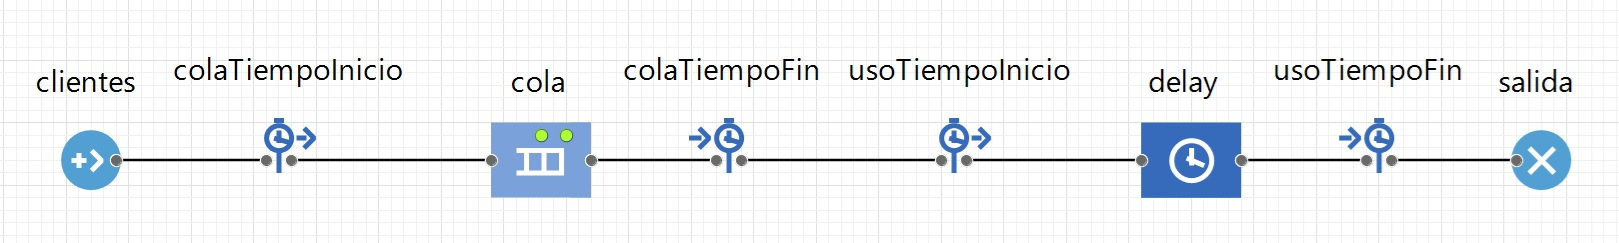
\includegraphics[width=\linewidth]{images/anylogic-colas-modelo}
  \caption{Bloques del modelo MM1 en Anylogic.}
\end{figure}

Para analizar el rendimiento del modelo, variamos la tasa de arribos ($T_a$) en base a la tasa de servicio ($T_s$), y
la capacidad de la cola ($cap$).

Realizaremos 10 simulaciones de 1000 clientes cada una y promediamos los siguientes estadísticos:
\begin{itemize}
    \item Promedio de clientes en el sistema ($q(n)+u(n)$)
    \item Cantidad de clientes en cola en promedio ($q(n)$)
    \item Demora promedio esperada en cola ($d(n)$)
    \item Tiempo promedio en el sistema ($d(n)+s(n)$)
    \item Ocupación del servidor ($u(n)*100\%$)
    \item Probabilidad de denegación del servicio. ($p(den)$)
    \item Probabilidad de encontrar n clientes en cola. ($p(Q(t)=n)\times100\%$)
\end{itemize}

Los primeros 5 fueron tabulados y el último fue graficado.

\subsubsection{$cap = 0$}

Los parámetros $d(n)$, $q(n)$ y $p(Q(t)=n)\times100\%$ no aplican cuando la capacidad de la cola es 0.
El promedio de clientes en sistema es en este caso, equivalente al factor de uso del servicio.

\begin{tabular}{||c||c|c|c||}
    \hline \hline
    ${T_a \over T_s}\times100\%$ [\%] & $d(n)+s(n)$ [min] & $u(n)\times100\%$ [\%] & $p(den)$ [\%] \\
    \hline \hline
    25 & $2,005$ & $19,823$ & $19,46$ \\
    \hline
    50 & $2,059$ & $33,656$ & $34,09$ \\
    \hline
    75 & $1,93$ & $42,212$ & $41,65$ \\
    \hline
    100 & $1,985$ & $49,165$ & $50,12$ \\
    \hline
    125 & $2,004$ & $55,434$ & $55,15$ \\
    \hline \hline
\end{tabular}

\subsubsection{$cap = 2$}

\begin{tabular}{||c||c|c|c|c|c|c||}
    \hline \hline
    ${T_a \over T_s}\times100\%$ [\%] & $q(n)+u(n)$ [min] & $q(n)$ [clientes] & $d(n)$ [min] & $d(n)+s(n)$ [min] & $u(n)\times100\%$ [\%] & $p(den)$ [\%] \\
    \hline \hline
    25 & $0,313$ & $0,068$ & $0,548$ & $2,54$ & $24,546$ & $1,26$ \\
    \hline
    50 & $0,739$ & $0,266$ & $1,148$ & $3,186$ & $47,27$ & $6,39$ \\
    \hline
    75 & $1,168$ & $0,524$ & $1,65$ & $3,681$ & $64,373$ & $15,71$ \\
    \hline
    100 & $1,499$ & $0,748$ & $2,014$ & $4,039$ & $75,164$ & $25,3$ \\
    \hline
    125 & $1,756$ & $0,934$ & $2,26$ & $4,246$ & $82,168$ & $32,93$ \\
    \hline \hline
\end{tabular}

\begin{figure}[H]
  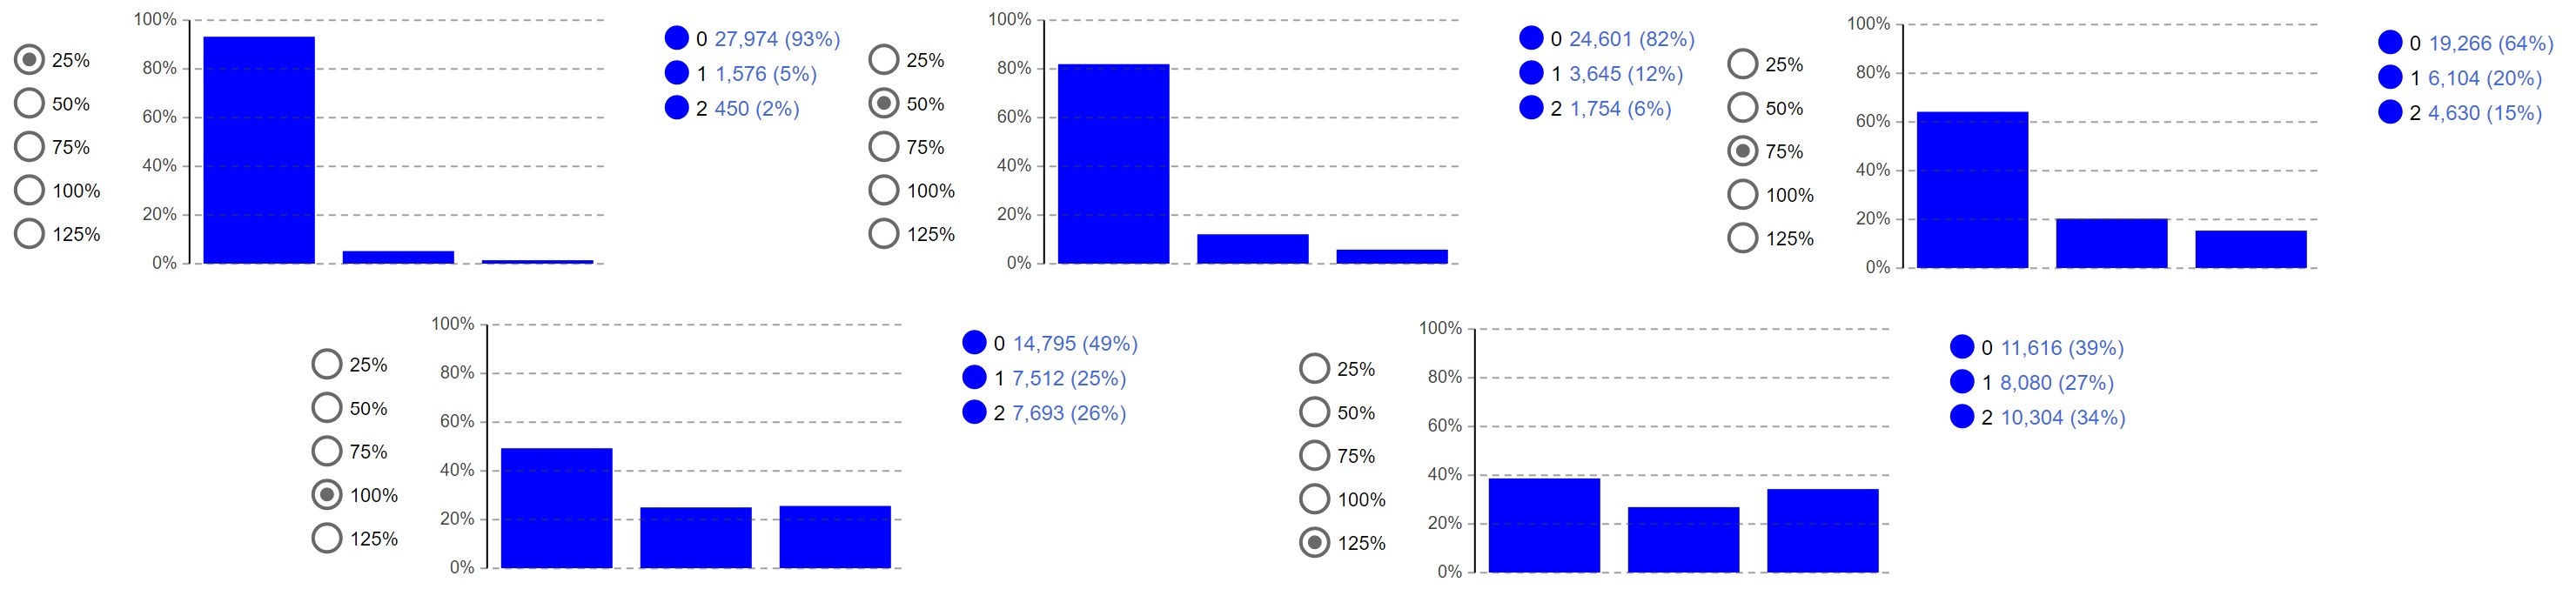
\includegraphics[width=\linewidth]{images/anylogic-colas-2}
  \caption{Probabilidad de encontrar n clientes en cola.}
\end{figure}

\subsubsection{$cap = 5$}

\begin{tabular}{||c||c|c|c|c|c|c||}
    \hline \hline
    ${T_a \over T_s}\times100\%$ [\%] & $q(n)+u(n)$ [min] & $q(n)$ [clientes] & $d(n)$ [min] & $d(n)+s(n) [min]$ & $u(n)\times100\%$ [\%] & $p(den)$ [\%] \\
    \hline \hline
    25 & $0,326$ & $0,079$ & $0,634$ & $2,069$ & $24,672$ & $0,01$ \\
    \hline
    50 & $0,917$ & $0,424$ & $1,7$ & $3,681$ & $49,263$ & $0,85$ \\
    \hline
    75 & $1,882$ & $1,18$ & $3,318$ & $5,289$ & $70,119$ & $4,9$ \\
    \hline
    100 & $3,122$ & $2,253$ & $5,234$ & $7,254$ & $86,914$ & $14,19$ \\
    \hline
    125 & $3,847$ & $2,917$ & $6,267$ & $8,266$ & $93,034$ & $25,23$ \\
    \hline \hline
\end{tabular}

\begin{figure}[H]
  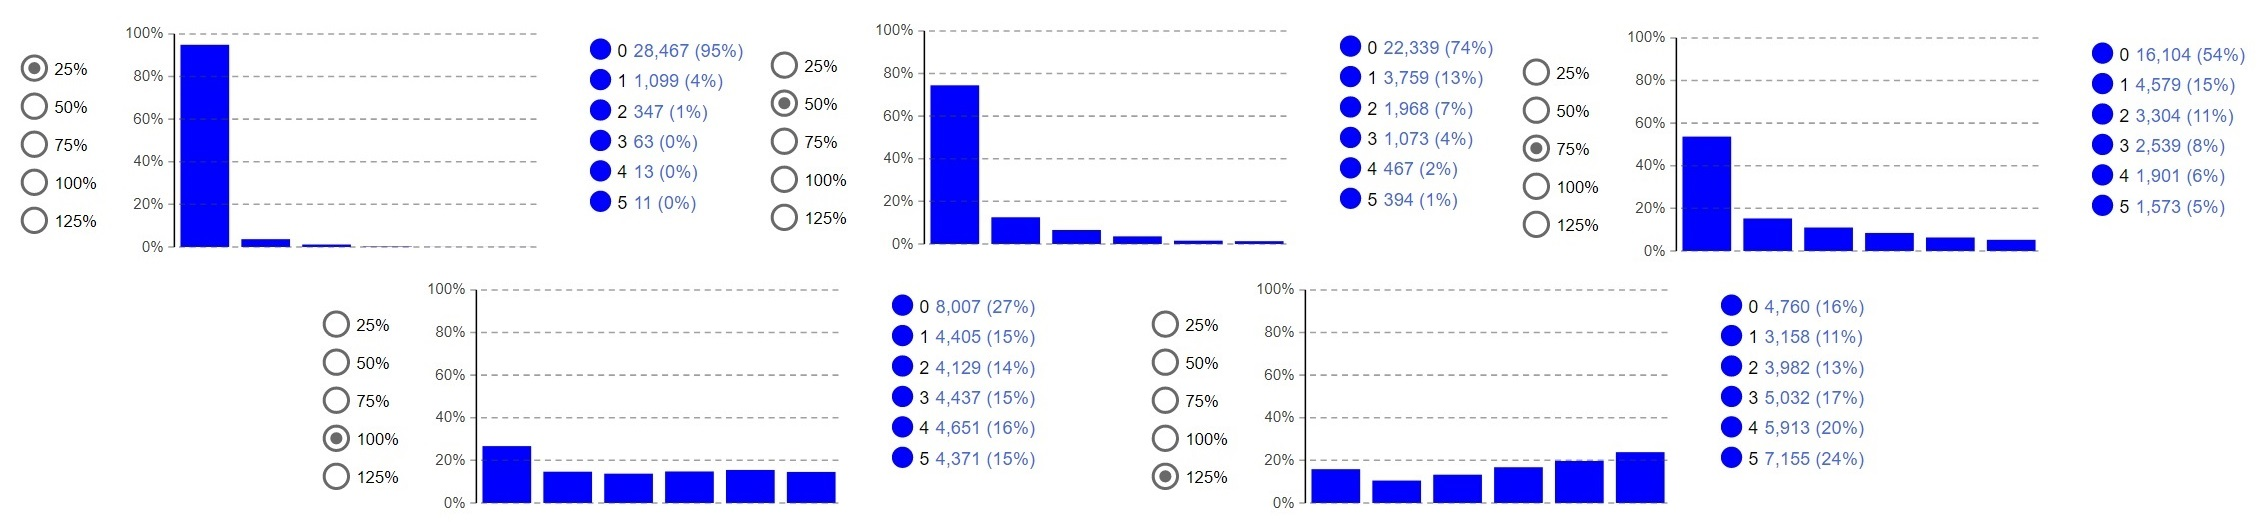
\includegraphics[width=\linewidth]{images/anylogic-colas-5}
  \caption{Probabilidad de encontrar n clientes en cola.}
\end{figure}

\subsubsection{$cap = 10$}

\begin{tabular}{||c||c|c|c|c|c|c||}
    \hline \hline
    ${T_a \over T_s}\times100\%$ [\%] & $q(n)+u(n)$ [min] & $q(n)$ [clientes] & $d(n)$ [min] & $d(n)+s(n) [min]$ & $u(n)\times100\%$ [\%] & $p(den)$ [\%] \\
    \hline \hline
    25 & $0,325$ & $0,08$ & $0,648$ & $2,631$ & $24,52$ & $0$ \\
    \hline
    50 & $1,032$ & $0,534$ & $2,15$ & $4,159$ & $49,816$ & $0,08$ \\
    \hline
    75 & $2,314$ & $1,593$ & $4,351$ & $6,332$ & $72,183$ & $0,64$ \\
    \hline
    100 & $5,294$ & $4,382$ & $9,62$ & $11,623$ & $91,217$ & $8.13$ \\
    \hline
    125 & $7,582$ & $6,606$ & $13.329$ & $15,296$ & $97.504$ & $19,65$ \\
    \hline \hline
\end{tabular}

\begin{figure}[H]
  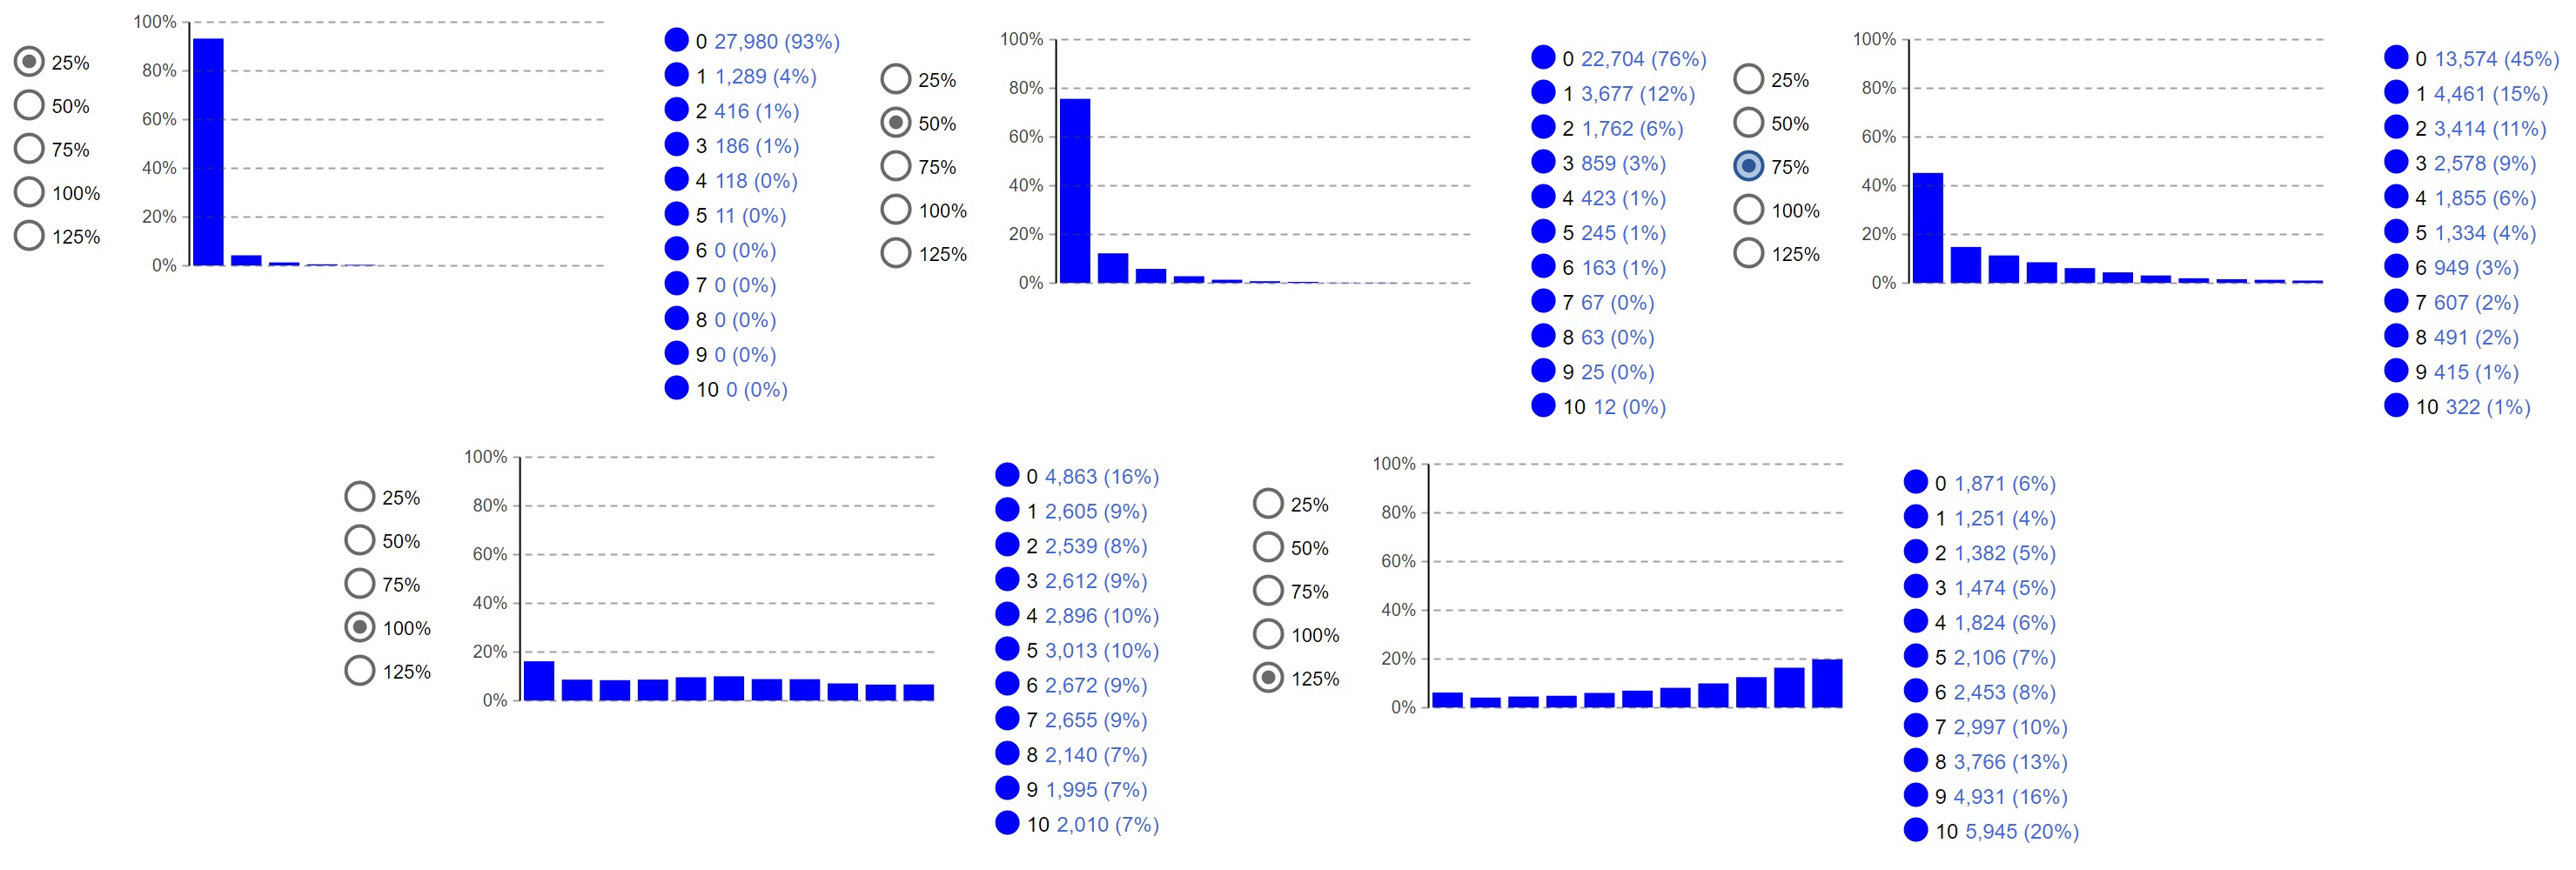
\includegraphics[width=\linewidth]{images/anylogic-colas-10}
  \caption{Probabilidad de encontrar n clientes en cola.}
\end{figure}

\subsubsection{$cap = 50$}

\begin{tabular}{||c||c|c|c|c|c|c||}
    \hline \hline
    ${T_a \over T_s}\times100\%$ [\%] & $q(n)+u(n)$ [min] & $q(n)$ [clientes] & $d(n)$ [min] & $d(n)+s(n) [min]$ & $u(n)\times100\%$ [\%] & $p(den)$ [\%] \\
    \hline \hline
    25 & $0,335$ & $0,085$ & $0,679$ & $2,686$ & $25,007$ & $0$ \\
    \hline
    50 & $1,039$ & $0,532$ & $2,099$ & $4,11$ & $50,7$ & $0$ \\
    \hline
    75 & $3,116$ & $2,368$ & $6,341$ & $8,358$ & $74,8$ & $0$ \\
    \hline
    100 & $22,932$ & $21,957$ & $45,615$ & $47,631$ & $97,42$ & $0,8$ \\
    \hline
    125 & $39,365$ & $38,37$ & $75,431$ & $77,386$ & $99,539$ & $13,41$ \\
    \hline \hline
\end{tabular}

\begin{figure}[H]
  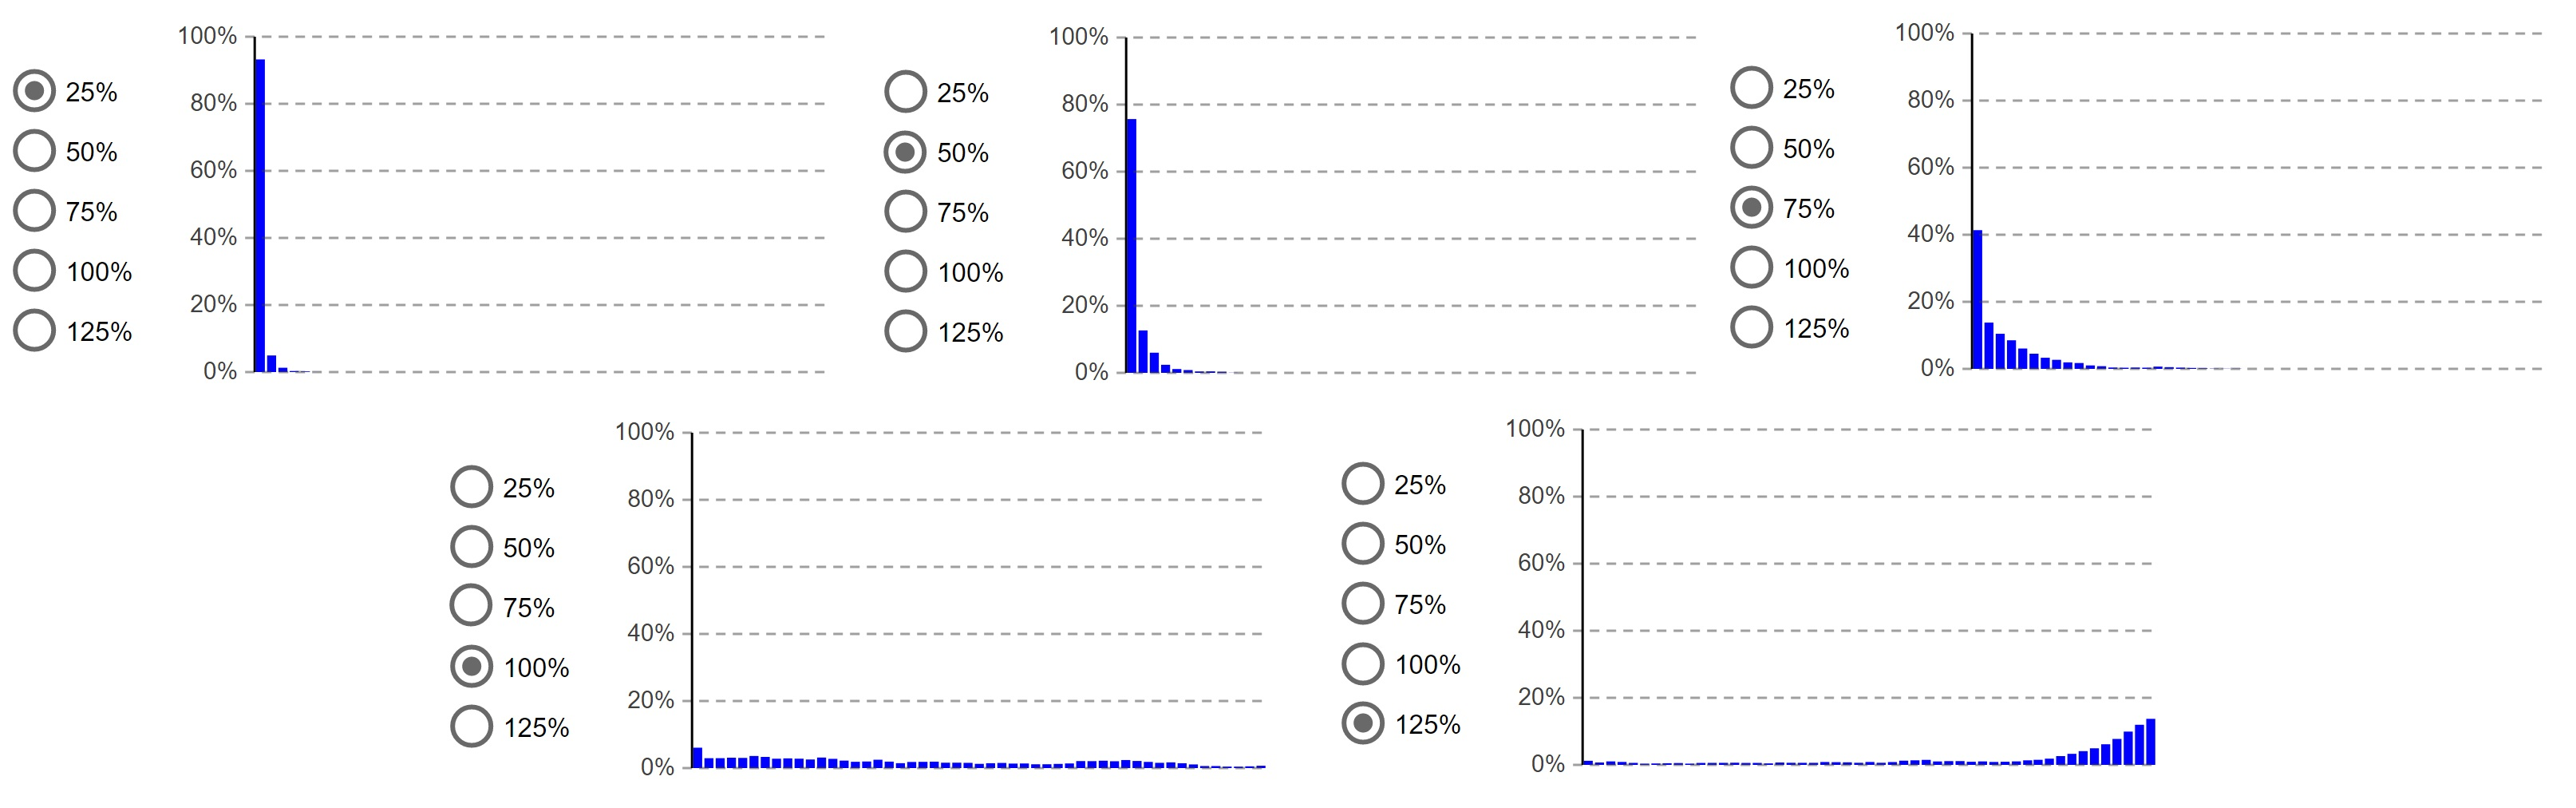
\includegraphics[width=\linewidth]{images/anylogic-colas-50}
  \caption{Probabilidad de encontrar n clientes en cola.}
\end{figure}

    \subsection{Modelo MM1 en Python}

Para analizar el rendimiento del modelo, variamos la tasa de arribos ($T_a$) en base a la tasa de servicio ($T_s$), y
la capacidad de la cola ($cap$).

Realizaremos 100 simulaciones de 1000 clientes cada una y promediamos los siguientes estadísticos:
\begin{itemize}
    \item Promedio de clientes en el sistema ($q(n)+u(n)$)
    \item Cantidad de clientes en cola en promedio ($q(n)$)
    \item Demora promedio esperada en cola ($d(n)$)
    \item Tiempo promedio en el sistema ($d(n)+s(n)$)
    \item Ocupación del servidor ($u(n)$)
    \item Probabilidad de denegación del servicio. ($p(den)$)
    \item Probabilidad de encontrar n clientes en cola. ($p(Q(t)=n)$)
\end{itemize}

Presentaremos los resultados obtenidos junto con sus intervalos de confianza del 95\%, obtenidos suponiendo que los mismos se distribuyen de manera normal, por el teorema central del límite, en el formato $valor \pm error$.

\subsubsection[cap = 0]{$cap = 0$}

Los parámetros $d(n)$, $q(n)$ y $p(Q(t)=n)$ no aplican cuando la capacidad de la cola es 0. El promedio de clientes en sistema es en este caso, equivalente al factor de uso del servicio.

\begin{tabular}{||c||c|c|c||}
    \hline \hline
    $\frac{T_a}{T_s}\times100\%$ [\%] & $d(n)+s(n)$ [min] & $u(n)\times100\%$ [\%] & $p(den)$ [\%] \\
    \hline \hline
    25 & $0.499 \pm 0.031$ & $19.897 \pm 1.504$ & $25.141 \pm 3.384$ \\
    \hline
    50 & $0.503 \pm 0.031$ & $33.437 \pm 1.899$ & $50.571 \pm 5.685$ \\
    \hline
    75 & $0.498 \pm 0.031$ & $42.698 \pm 2.11$ & $74.62 \pm 7.204$ \\
    \hline
    100 & $0.5 \pm 0.031$ & $49.982 \pm 2.341$ & $99.75 \pm 8.792$ \\
    \hline
    125 & $0.501 \pm 0.033$ & $55.659 \pm 2.3$ & $$ \\
    \hline \hline
\end{tabular}

\subsubsection[cap = 2]{$cap = 2$}

\begin{tabular}{||c||c|c|c|c|c|c||}
    \hline \hline
    $\frac{T_a}{T_s}\times100\%$ [\%] & $q(n)+u(n)$ [min] & $q(n)$ [clientes] & $d(n)$ [min] & $d(n)+s(n)$ [min] & $u(n)\times100\%$ [\%] & $p(den)$ [\%] \\
    \hline \hline
    25 & $$ & $$ & $$ & $$ & $$ & $$ \\
    \hline
    50 & $$ & $$ & $$ & $$ & $$ & $$ \\
    \hline
    75 & $$ & $$ & $$ & $$ & $$ & $$ \\
    \hline
    100 & $$ & $$ & $$ & $$ & $$ & $$ \\
    \hline
    125 & $$ & $$ & $$ & $$ & $$ & $$ \\
    \hline \hline
\end{tabular}

\begin{figure}[H]
  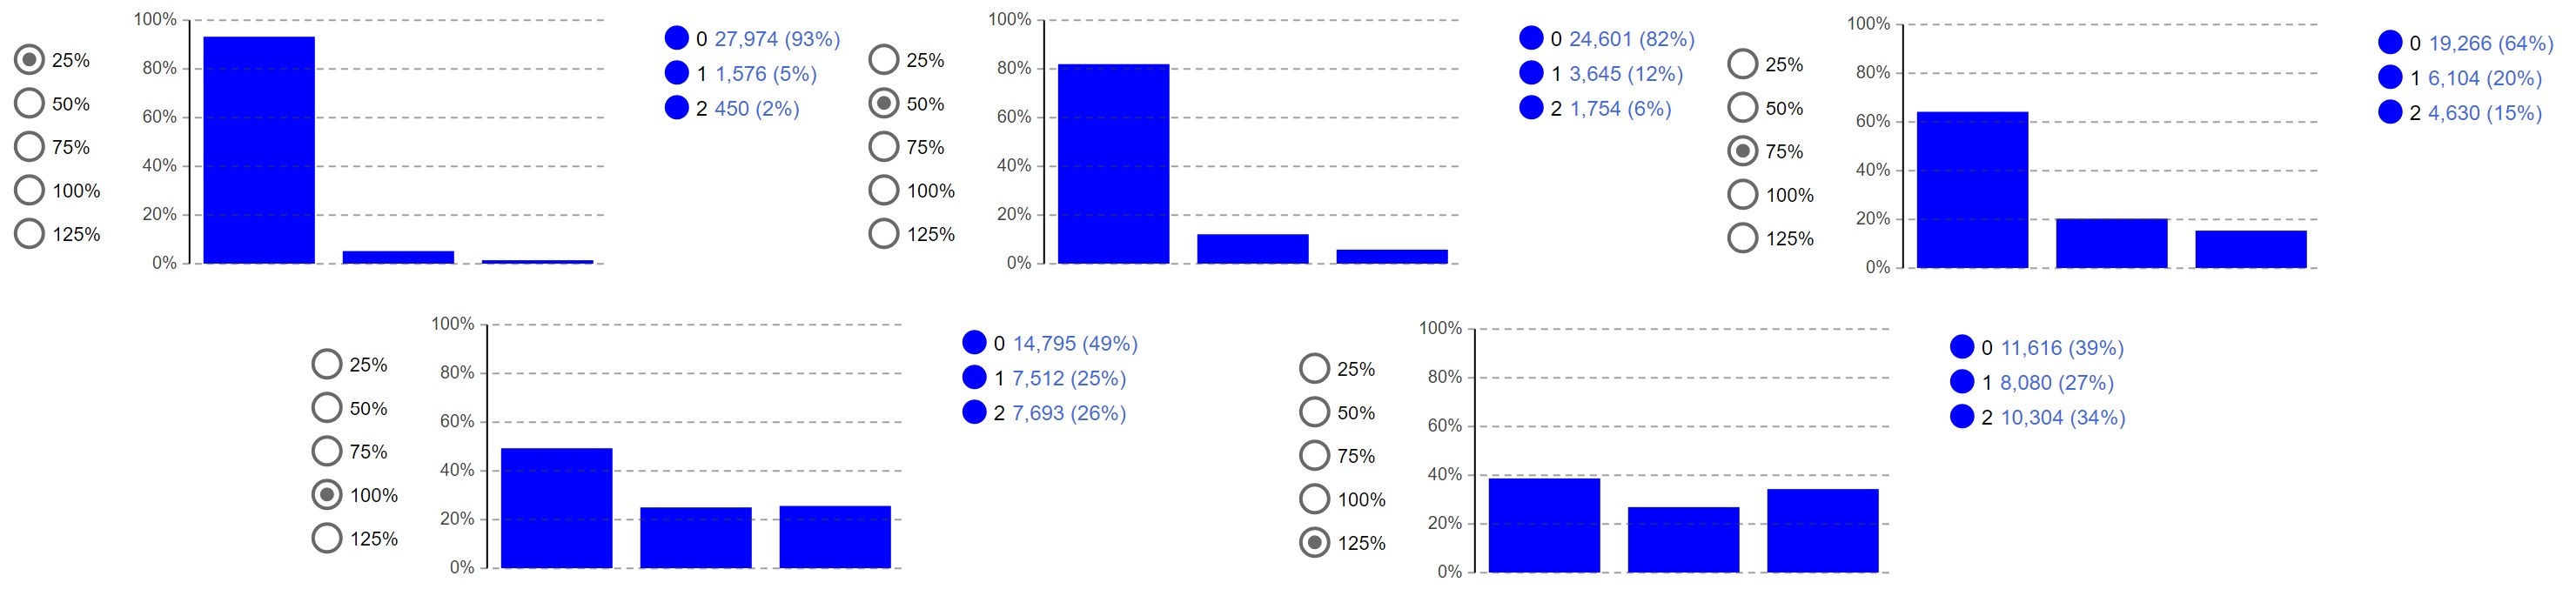
\includegraphics[width=\linewidth]{images/anylogic-colas-2}
  \caption{Probabilidad de encontrar n clientes en cola.}
\end{figure}

\subsubsection[cap = 5]{$cap = 5$}

\begin{tabular}{||c||c|c|c|c|c|c||}
    \hline \hline
    $\frac{T_a}{T_s}\times100\%$ [\%] & $q(n)+u(n)$ [min] & $q(n)$ [clientes] & $d(n)$ [min] & $d(n)+s(n) [min]$ & $u(n)\times100\%$ [\%] & $p(den)$ [\%] \\
    \hline \hline
    25 & $$ & $$ & $$ & $$ & $$ & $$ \\
    \hline
    50 & $$ & $$ & $$ & $$ & $$ & $$ \\
    \hline
    75 & $$ & $$ & $$ & $$ & $$ & $$ \\
    \hline
    100 & $$ & $$ & $$ & $$ & $$ & $$ \\
    \hline
    125 & $$ & $$ & $$ & $$ & $$ & $$ \\
    \hline \hline
\end{tabular}

\begin{figure}[H]
  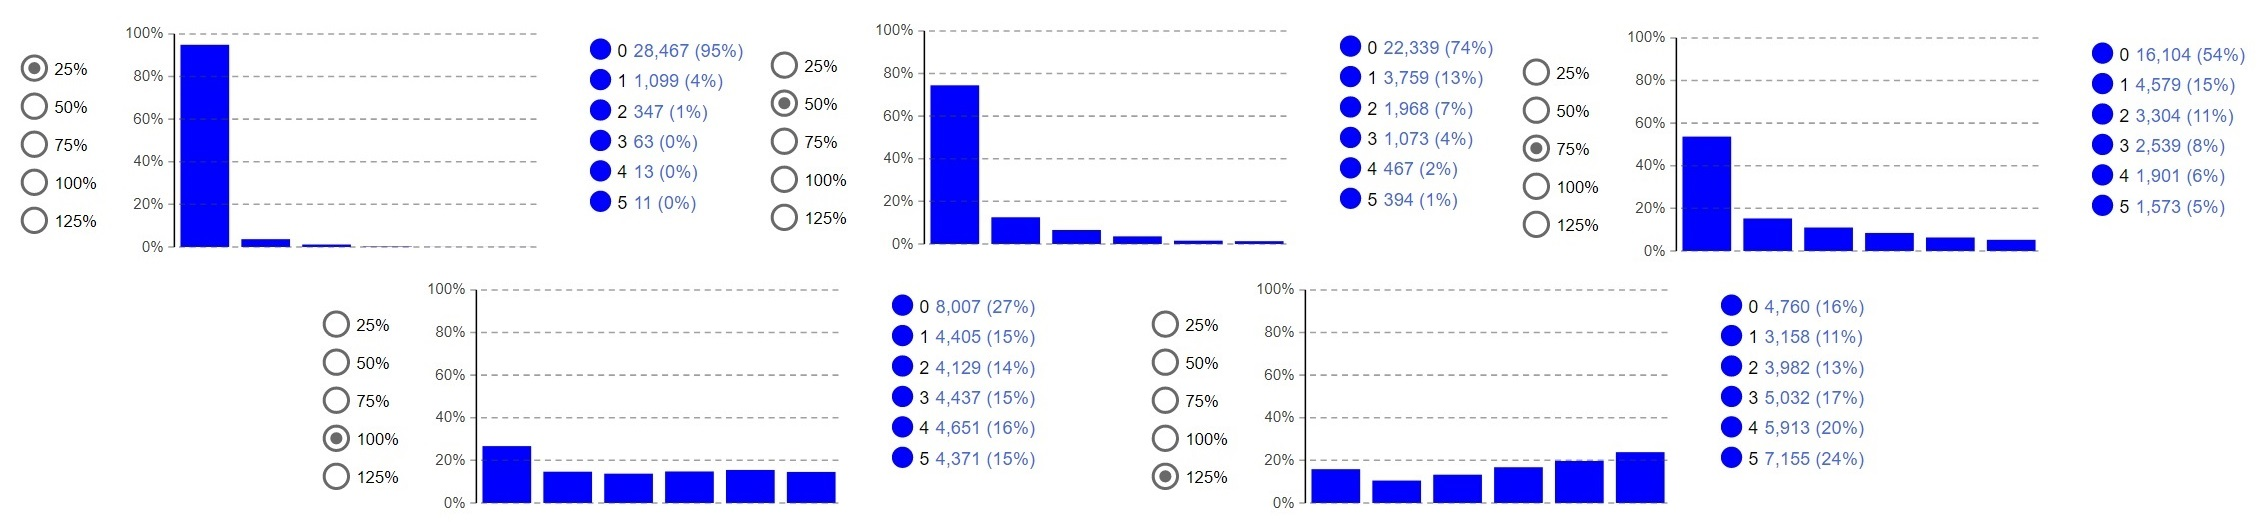
\includegraphics[width=\linewidth]{images/anylogic-colas-5}
  \caption{Probabilidad de encontrar n clientes en cola.}
\end{figure}

\subsubsection[cap = 10]{$cap = 10$}

\begin{tabular}{||c||c|c|c|c|c|c||}
    \hline \hline
    $\frac{T_a}{T_s}\times100\%$ [\%] & $q(n)+u(n)$ [min] & $q(n)$ [clientes] & $d(n)$ [min] & $d(n)+s(n) [min]$ & $u(n)\times100\%$ [\%] & $p(den)$ [\%] \\
    \hline \hline
    25 & $$ & $$ & $$ & $$ & $$ & $$ \\
    \hline
    50 & $$ & $$ & $$ & $$ & $$ & $$ \\
    \hline
    75 & $$ & $$ & $$ & $$ & $$ & $$ \\
    \hline
    100 & $$ & $$ & $$ & $$ & $$ & $$ \\
    \hline
    125 & $$ & $$ & $$ & $$ & $$ & $$ \\
    \hline \hline
\end{tabular}

\begin{figure}[H]
  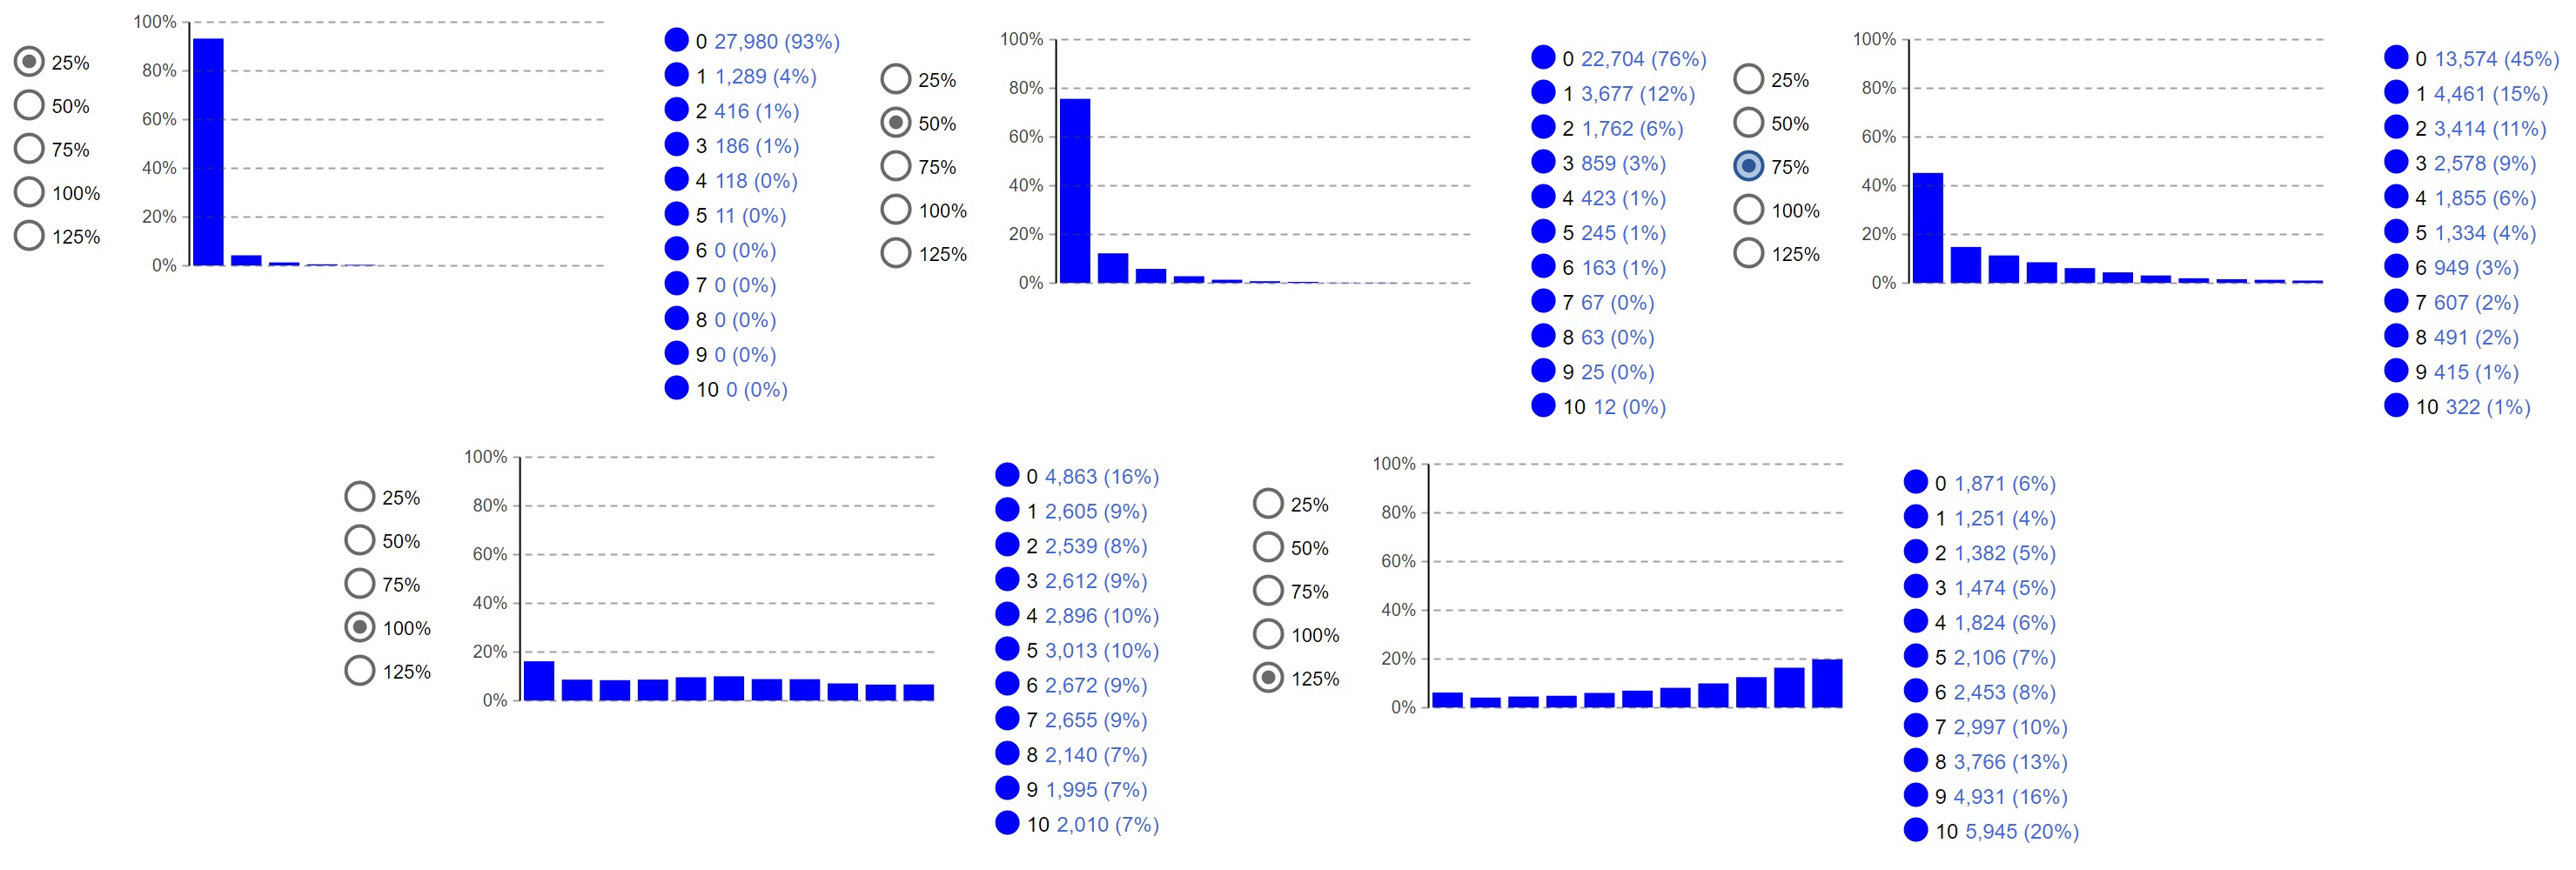
\includegraphics[width=\linewidth]{images/anylogic-colas-10}
  \caption{Probabilidad de encontrar n clientes en cola.}
\end{figure}

\subsubsection[cap = 50]{$cap = 50$}

\begin{tabular}{||c||c|c|c|c|c|c||}
    \hline \hline
    $\frac{T_a}{T_s}\times100\%$ [\%] & $q(n)+u(n)$ [min] & $q(n)$ [clientes] & $d(n)$ [min] & $d(n)+s(n) [min]$ & $u(n)\times100\%$ [\%] & $p(den)$ [\%] \\
    \hline \hline
    25 & $$ & $$ & $$ & $$ & $$ & $$ \\
    \hline
    50 & $$ & $$ & $$ & $$ & $$ & $$ \\
    \hline
    75 & $$ & $$ & $$ & $$ & $$ & $$ \\
    \hline
    100 & $$ & $$ & $$ & $$ & $$ & $$ \\
    \hline
    125 & $$ & $$ & $$ & $$ & $$ & $$ \\
    \hline \hline
\end{tabular}

\begin{figure}[H]
  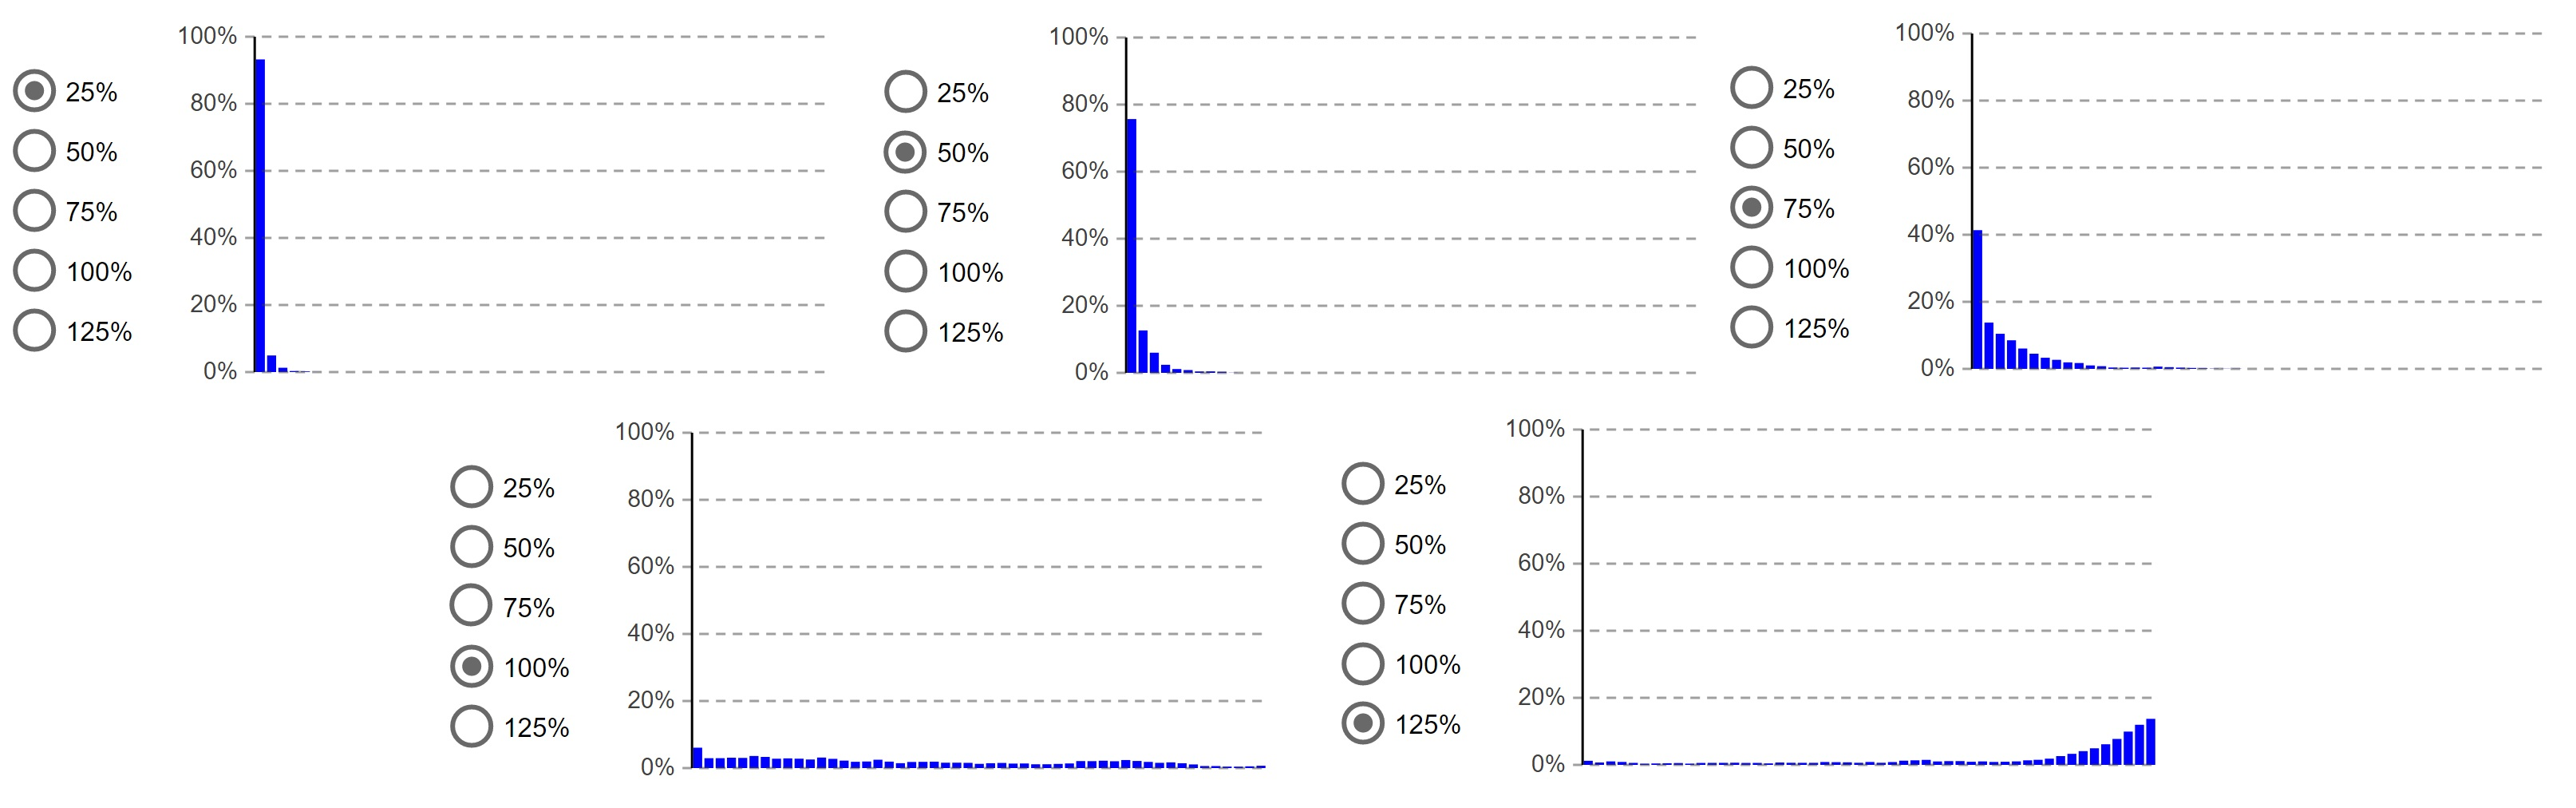
\includegraphics[width=\linewidth]{images/anylogic-colas-50}
  \caption{Probabilidad de encontrar n clientes en cola.}
\end{figure}

\subsubsection[cap = ∞]{$cap = \infty$}

En este caso no tenemos tope de clientes en la cola, entonces no hay probabilidad de denegación.

\begin{itemize}
    \item Promedio de clientes en el sistema ($q(n)+u(n)$)
    \item Cantidad de clientes en cola en promedio ($q(n)$)
    \item Demora promedio esperada en cola ($d(n)$)
    \item Tiempo promedio en el sistema ($d(n)+s(n)$)
    \item Ocupación del servidor ($u(n)*100\%$)
\end{itemize}

\begin{tabular}{||c||c|c|c|c|c|c||}
    \hline \hline
    $\frac{T_a}{T_s}\times100\%$ [\%] & $q(n)+u(n)$ [min] & $q(n)$ [clientes] & $d(n)$ [min] & $d(n)+s(n) [min]$ & $u(n)\times100\%$ [\%]\\
    \hline \hline
    25 & $0,331$ & $0,082$ & $0,653$ & $2,637$ & $24,866$ \\
    \hline
    50 & $0,995$ & $0,496$ & $1,978$ & $3,981$ & $49,949$ \\
    \hline
    75 & $2,924$ & $2,176$ & $5,778$ & $7,778$ & $74,845$ \\
    \hline
    100 & $23,853$ & $22,892$ & $45,548$ & $47,546$ & $96,121$ \\
    \hline
    125 & $127,97$ & $126,975$ & $203,476$ & $205,469$ & $99,563$ \\
    \hline \hline
\end{tabular}

\begin{figure}[H]
  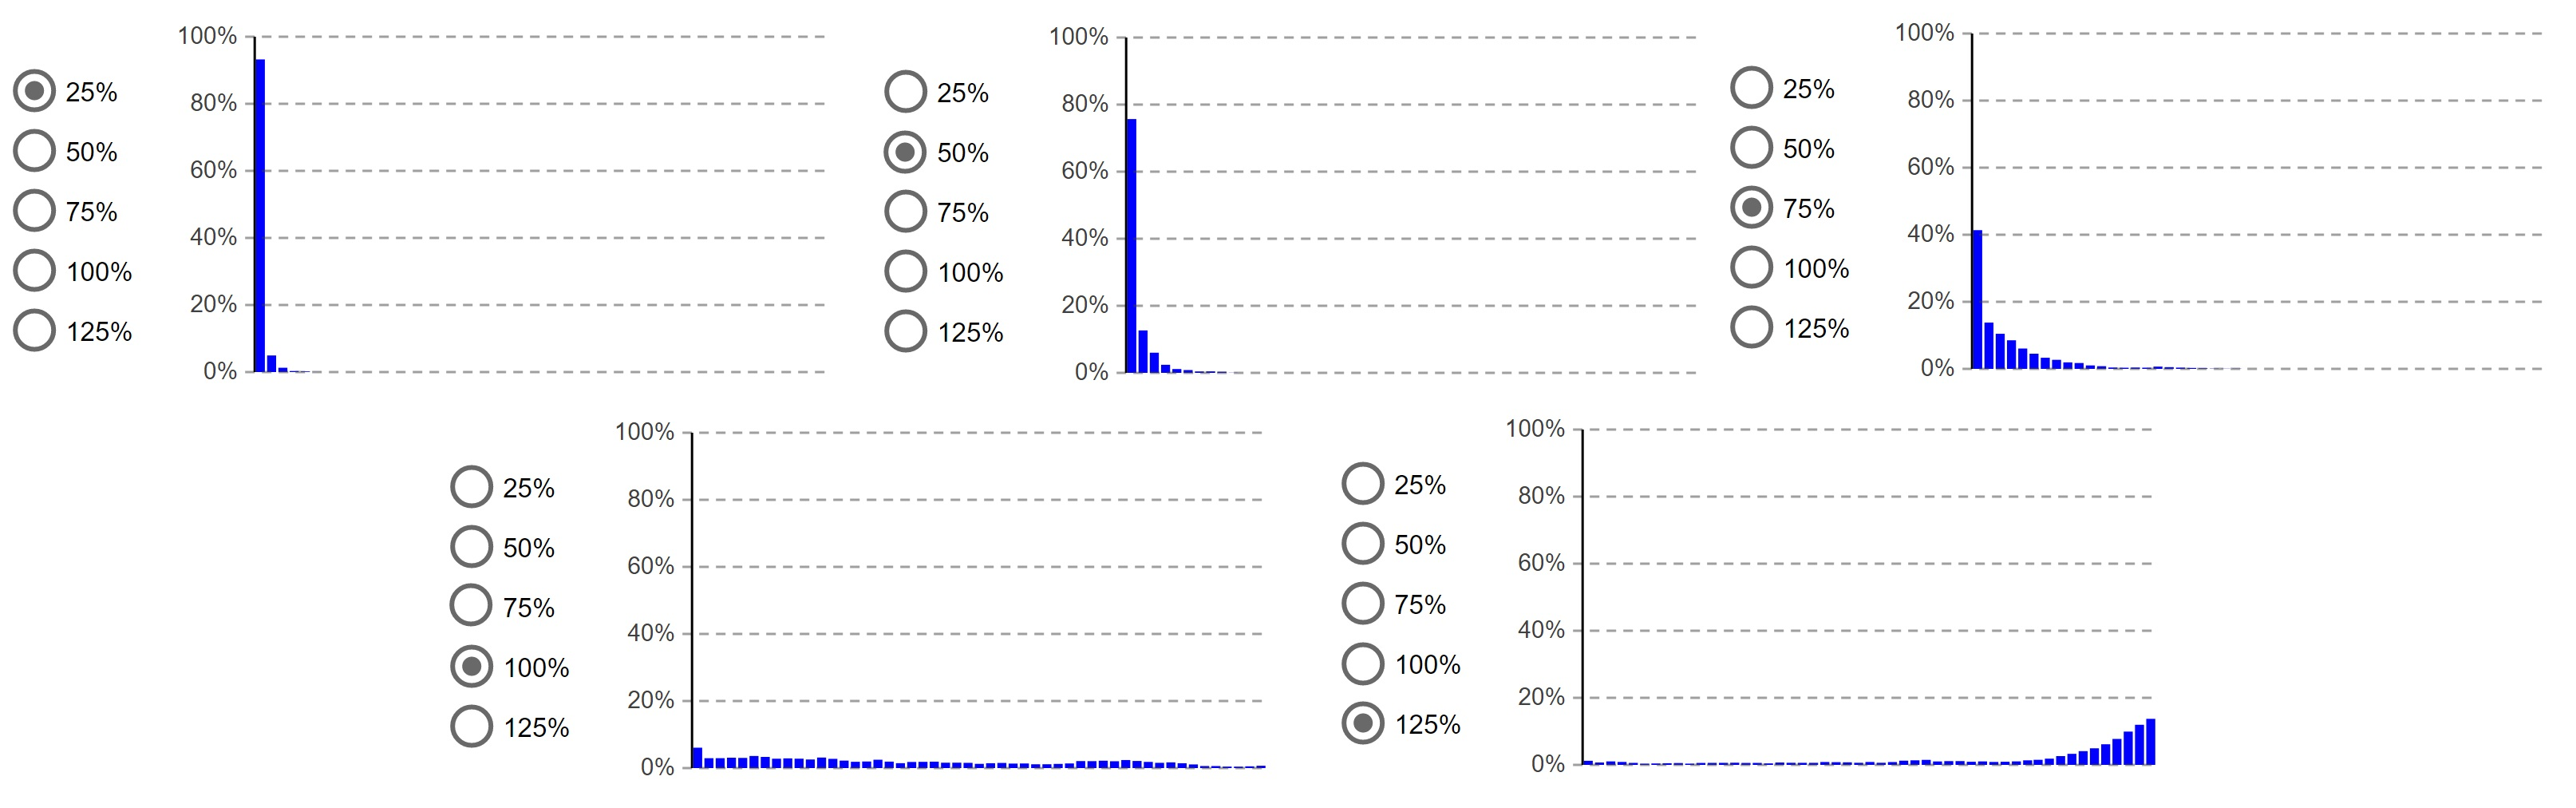
\includegraphics[width=\linewidth]{images/anylogic-colas-50}
  \caption{Probabilidad de encontrar n clientes en cola.}
\end{figure}


    \subsection{Modelo de inventario en Python}

En esta simulación se realizarán las corridas del sistema en base a los eventos correspondientes a las distintas acciones de un inventario.
El funcionamiento del sistema desarrollado consta de eventos que surgen por meses donde la demanda cambia en base a una distribución de probabilidad.
Cada cierto tiempo se realiza la evaluación del inventario con sus existencias o faltantes para poder tomar acciones que permitan cubrir la demanda según una política de inventario determinada $(s, S)$.
En caso de que ante la demanda el modelo de inventario tenga una existencia menor al nivel inferior de inventario $s$, entonces se programa un pedido con la cantidad necesaria para completar hasta el nivel superior $S$, esto es $S - I$, para que luego de unos días llegue y el inventario se reponga.
Caso contrario, si el nivel de inventario es mayor o igual que $s$, sigue funcionando de manera habitual.

Para esto se tendrán en cuenta los siguientes parámetros con los que se contará para poder llegar a nuestros objetivos:
\begin{itemize}
    \item Política de inventario $(s, S)$: niveles inferior y superior de inventario que determinan a partir de qué punto realizar un pedido y en qué cantidad.
    \item Nivel inicial de inventario: en nuestro caso igual a $60$ unidades.
    \item Costo de mantenimiento ($h$): precio por el cual se mantiene cada unidad en stock, $\$ 1$ para nuestro caso.
    \item Costo inicial de envío ($K$): costo fijo en el que se incurre cada vez que se hace un pedido, $\$ 32$ (cuando la cantidad pedida $Z > 0$, si no $\$ 0$) para nuestro caso.
    \item Costo incremental de envío ($i$): costo adicional por unidad pedida, $\$ 3$ para nuestro caso.
    \item Costo de orden ($C_o(Z)$): costo de realizar una orden de compra, $C_o(Z) = K + iZ$.
    \item Costo de faltante ($\pi$): costo por la falta de stock, $\$ 5$ para nuestro caso.
    \item Tardanza de la reposición: tiempo que tarda en arribar un pedido para reponer stock, en nuestro caso es una variable aleatoria que se distribuye de manera uniforme entre 0.5 y 1 mes.
    \item Tiempo medio entre demandas (meses): variable aleatoria con distribución exponencial, $\nicefrac{1}{\lambda} = 0.1$ en nuestro caso ($\lambda = 10$ demandas/mes).
    \item Distribución de la demanda: en nuestro caso $D=\left\{ \begin{array}{lcc}
            1 &   c.p.  & 1/6 \\
            \\ 2 &  c.p. & 1/3 \\
            \\ 3 &  c.p. & 1/3 \\
            \\ 4 &  c.p.  & 1/6
  \end{array}
  \right.$.
    \item Criterio de finalización: en nuestro caso es por el tiempo de la simulación, $t = 120$ meses, es decir 10 años.
\end{itemize}

Para poder llevar a cabo la simulación, emplearemos las siguientes variables de estado y estadísticas:
\begin{itemize}
    \item Nivel de inventario: el nivel actual del inventario.
    \item Costo total de pedido: el costo de pedido acumulado actual.
    \item Área de existencia: área debajo del nivel de inventario real a lo largo del tiempo.
    \item Área de escasez: área debajo del nivel de inventario faltante a lo largo del tiempo.
\end{itemize}

Finalmente, el sistema calcula los costos mencionados anteriormente para poder analizar el estado de los costos del inventario, hacer comparaciones y extraer conclusiones que permitan tomar decisiones.

Para analizar el rendimiento del modelo, variamos la política de inventario $(s, S)$, dado que es el principal factor que la empresa puede modificar y sobre el cual podrá tomar decisiones.

Realizaremos 100 simulaciones, de 120 meses cada una como se ha mencionado anteriormente y promediaremos los siguientes estadísticos:
\begin{itemize}
    \item Costo de orden promedio ($\bar{C}_{o}$)
    \item Costo de mantenimiento promedio ($h \bar{I}^{+}$)
    \item Costo de faltante promedio ($\pi \bar{I}^{-}$)
    \item Costo total promedio ($\bar{C}_{T} = \bar{C}_{o} + h \bar{I}^{+} + \pi \bar{I}^{-}$)
\end{itemize}

Presentaremos los resultados obtenidos junto con sus intervalos de confianza del 95\%, obtenidos suponiendo que los mismos se distribuyen de manera normal, por el teorema central del límite, en el formato $valor \pm error$.

\begin{tabular}{||c||c|c|c|c||}
    \hline \hline
    Política $(s, S)$ & $\bar{C}_{o}$ [\$/mes] & $h \bar{I}^{+}$ [\$/mes] & $\pi \bar{I}^{-}$ [\$/mes] & $\bar{C}_{T}$ [\$/mes] \\
    \hline \hline
    $(20, 40)$ & $97.428 \pm 5.639$ & $9.277 \pm 1.043$ & $17.693 \pm 4.08$ & $124.398 \pm 7.457$ \\
    $(20, 60)$ & $88.624 \pm 4.921$ & $17.531 \pm 1.581$ & $12.926 \pm 3.972$ & $119.081 \pm 6.545$ \\
    $(20, 80)$ & $85.022 \pm 5.32$ & $26.941 \pm 2.093$ & $9.653 \pm 3.539$ & $121.615 \pm 6.333$ \\
    $(20, 100)$ & $83.098 \pm 5.35$ & $36.777 \pm 2.074$ & $7.336 \pm 2.821$ & $127.211 \pm 5.857$ \\
    $(40, 60)$ & $98.196 \pm 5.963$ & $25.615 \pm 1.484$ & $1.797 \pm 1.253$ & $125.608 \pm 5.411$ \\
    $(40, 80)$ & $88.739 \pm 5.041$ & $35.226 \pm 2.123$ & $1.342 \pm 1.11$ & $125.307 \pm 4.299$ \\
    $(40, 100)$ & $85.31 \pm 5.175$ & $45.12 \pm 2.393$ & $1.094 \pm 1.037$ & $131.523 \pm 4.598$ \\
    $(60, 80)$ & $99.073 \pm 6.08$ & $45.117 \pm 1.804$ & $0.075 \pm 0.204$ & $144.264 \pm 4.979$ \\
    $(60, 100)$ & $89.9 \pm 5.195$ & $54.423 \pm 2.206$ & $0.055 \pm 0.177$ & $144.378 \pm 3.938$ \\
    \hline \hline
\end{tabular}

    \subsection{Modelo de Inventario en AnyLogic}
\label{subsec:modelo-de-inventario-en-anylogic}
\begin{figure}[H]
    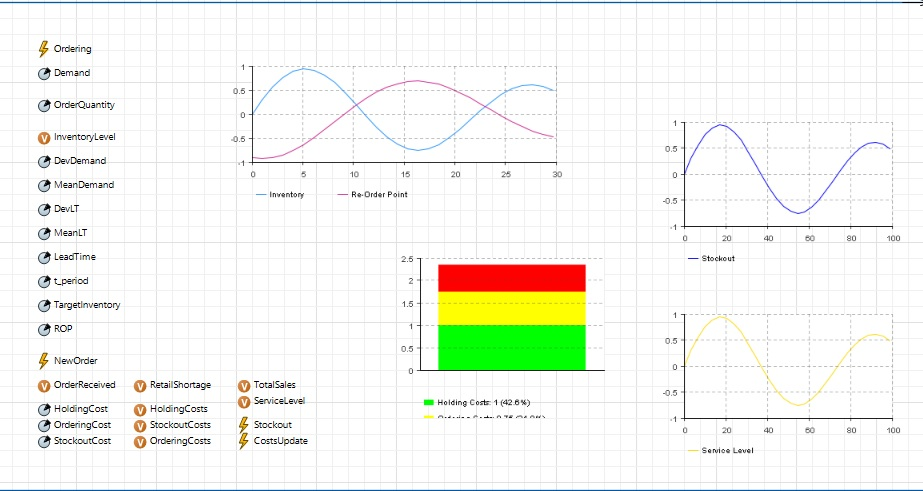
\includegraphics[width=\linewidth]{images/anylogic-inventario}
    \caption{Modelo de Inventario con sus parámetros,variables y eventos utilizados en Anygic.}
\end{figure}

Como podemos ver, hay ciertos parámetros que ya hemos utilizados en el modelo realizado en Python, pero fué necesario además agregar nuevos para poder utilizarlos con distintas funcionalidades.

Comenzando por el evento "Ordering" el cual nos permite programar los reabastecimientos del inventario a través de dos parámetros: (demand y order quantity). Además agregamos una variable llamada invetoryLevel la cual analizaremos con una linea de tiempo.

Este es un evento cíclico con un tiempo de recurrencia de un día.

Suponiendo que la demanda diaria y/o el tiempo de entrega se distribuyen normalmente.
Necesitamos definir más  parámetros para el tiempo de entrega, la demanda media, el tiempo de entrega promedio, la desviación estándar de la demanda y la desviación estándar del tiempo de entrega.

Para el sistema de revisión periódica, reabastecemos en fechas fijas, por lo que solo modificamos el tiempo de recurrencia del evento “Ordering” definiéndolo a través del parámetro "t\_period".

Para el sistema de revisión continua, la regla de reabastecimiento se puede definir con la ayuda del punto de pedido (ROP).

Además incluiremos stock de seguridad en nuestro modelo.
Para modelar el tiempo de entrega, definimos el evento "NewOrder" y la variable "OrderReceived de tipo "Booleano" (con valor inicial "false") y vuelva a escribir la regla de reposición en el evento "Ordering".

Si el nivel de inventario alcanza el punto de pedido, se genera un nuevo pedido de reabastecimiento el cual llegará en X días definidos en el parámetro LeadTime.
Es por eso que dejamos que el evento "NewOrder" comience en X días.
En el momento de la entrada del pedido y el aumento del nivel de inventario, la variable lógica "OrderReceived" toma el valor "false". Esto significa que no hay otras órdenes
recibidas por nuestro proveedor.
El siguiente pedido se generará cuando el nivel de inventario vuelva a alcanzar el punto de pedido.

Para estimar la eficiencia de las diferentes políticas de pedidos, necesitamos estimar los costos de mantenimiento de inventario, pedidos y agotamiento de existencias.
Primero, se necesitan nuevos parámetros y variables para estos tres tipos de costos. En segundo lugar, los diagramas deben construirse como gráficos de barras y diagramas de tiempo.
Definimos tres nuevos parámetros “HoldingCost”, “OrderingCost” y “StockoutCosts” y tres nuevas variables de los mismos. Es necesario definir otras tres nuevas variables, "ServiceLevel", "TotalSales" y "RetailShortage".

Los costos, la escasez y el nivel de servicio se actualizan en el evento "CostsUpdate".

A continuación se realizarán 10 simulaciones de 30 días cada una, donde se llevarán a cabo las mediciones de las siguientes variables:
\begin{itemize}
    \item Costo de Orden
    \item Costo de Mantenimiento
    \item Costo de Faltante
    \item Costo Total
\end{itemize}

\begin{figure}[H]
    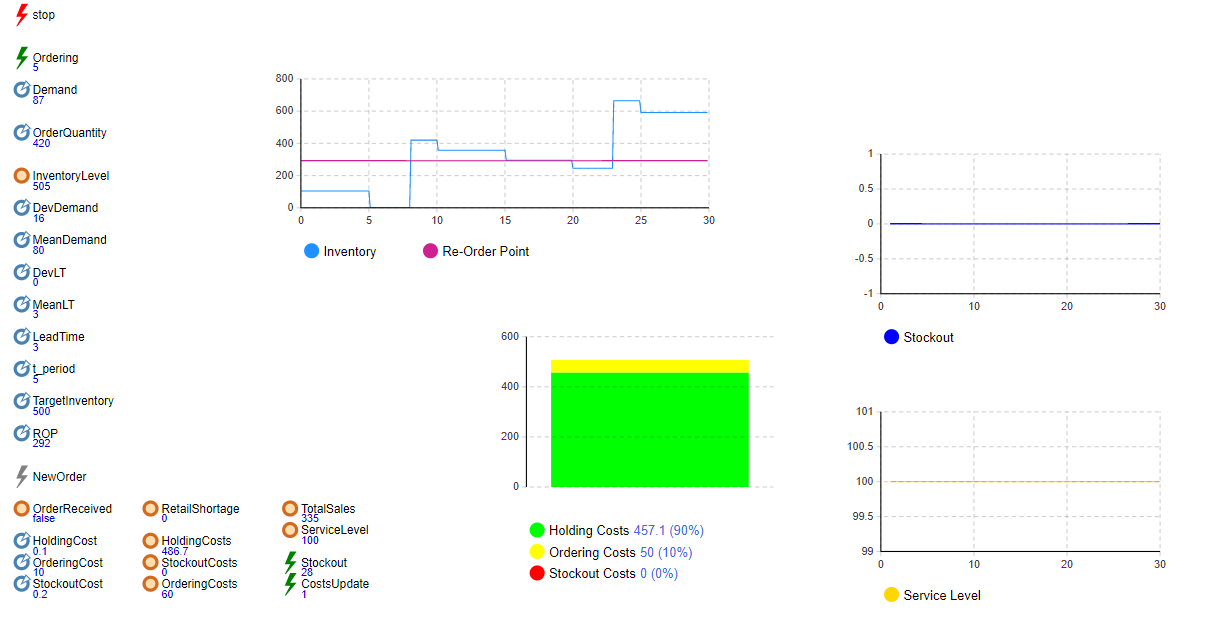
\includegraphics[width=\linewidth]{images/img1invent}
    \caption{Simulación 1. Orden de compra alto.}
\end{figure}

\begin{figure}[H]
    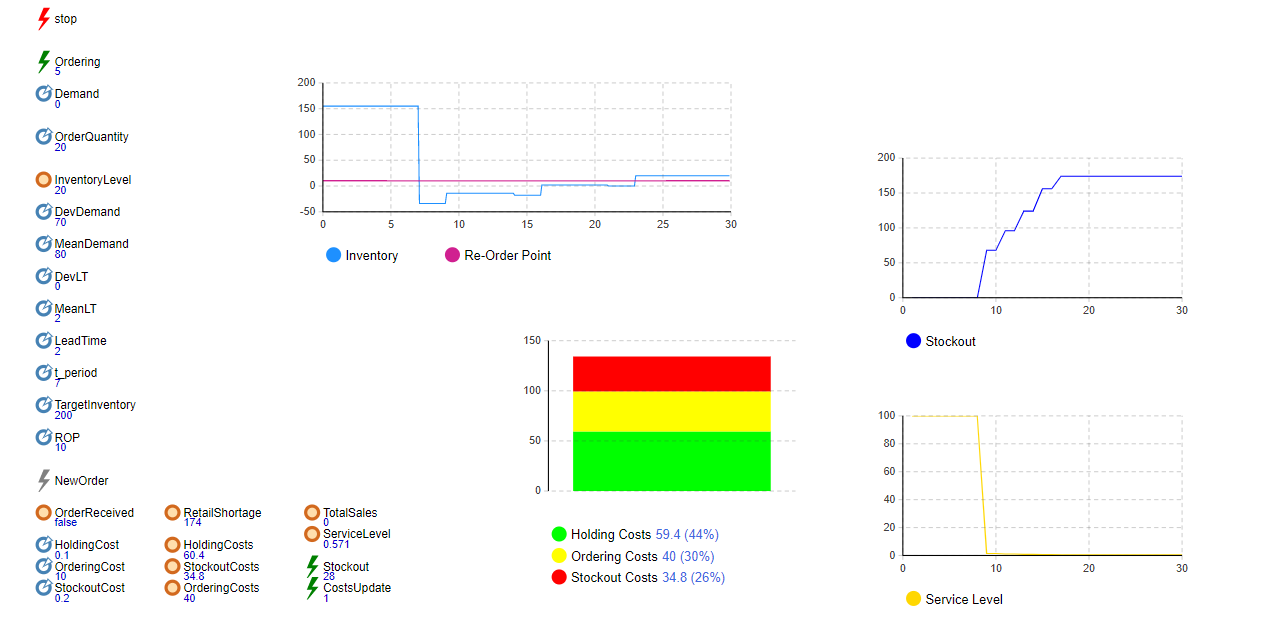
\includegraphics[width=\linewidth]{images/img2invent}
    \caption{Simulación 2. Orden de compra y ROP bajo.}
\end{figure}

\begin{figure}[H]
    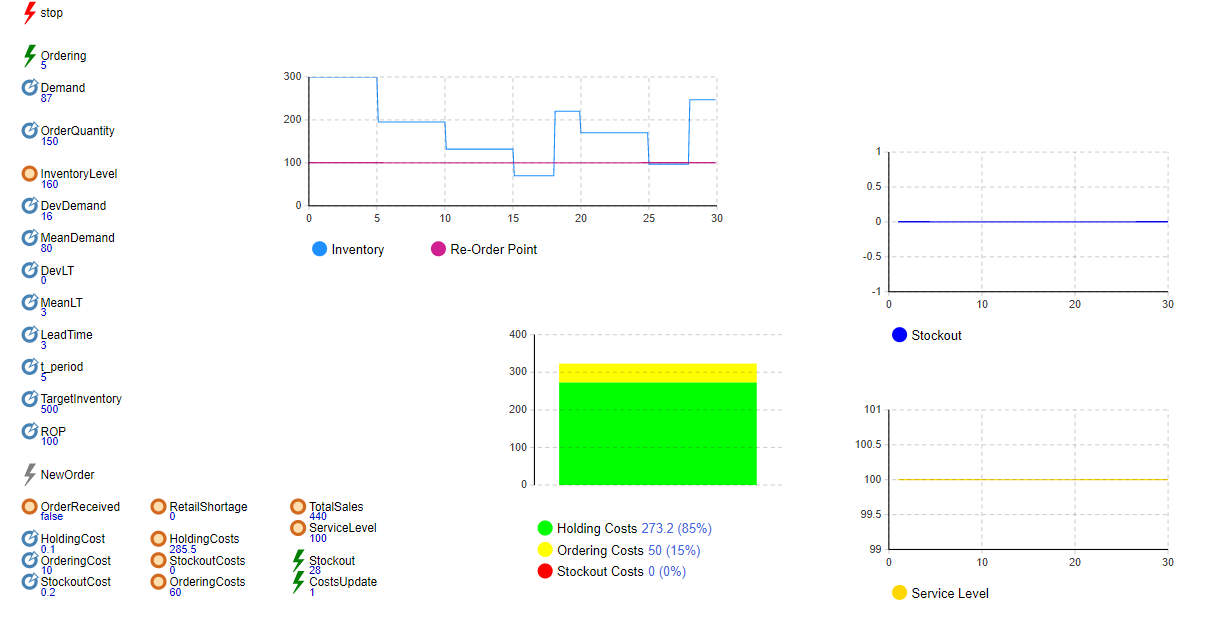
\includegraphics[width=\linewidth]{images/img3invent}
    \caption{Simulación 3. Cantidad inicial alta y ROP a un tercio de la cantidad inicial.}
\end{figure}

\begin{figure}[H]
    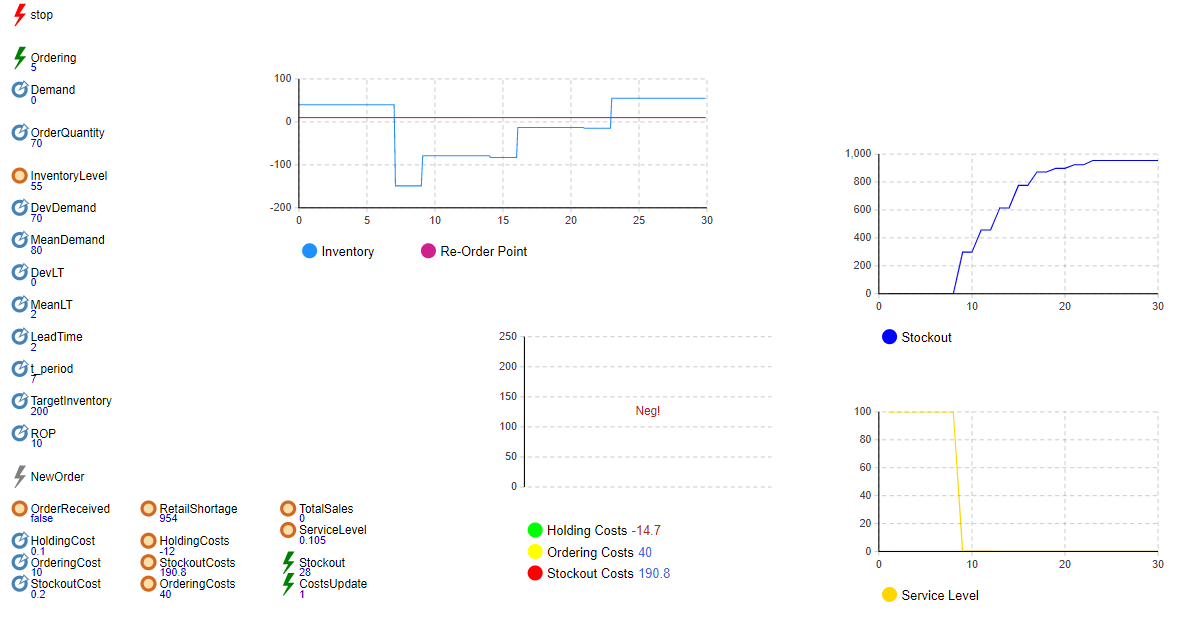
\includegraphics[width=\linewidth]{images/img4invent}
    \caption{Simulación 4. Gran falta de stock.}
\end{figure}

\begin{figure}[H]
    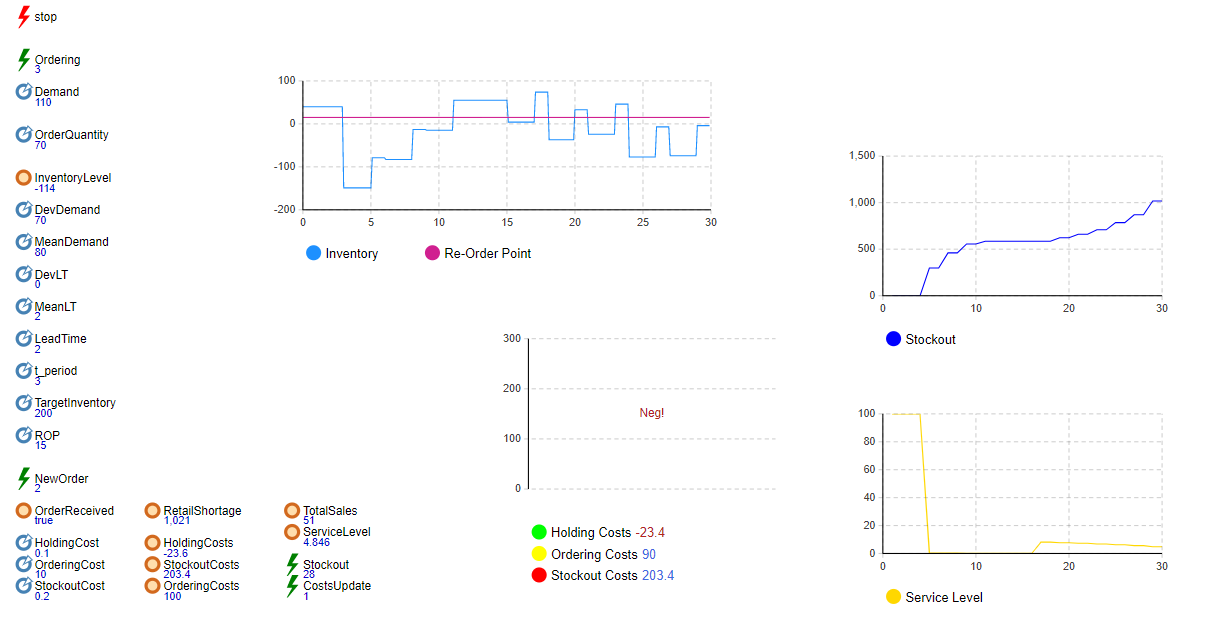
\includegraphics[width=\linewidth]{images/img5invent}
    \caption{Simulación 5. Gran falta de stock con mayor velocidad de recepción.}
\end{figure}

\begin{figure}[H]
    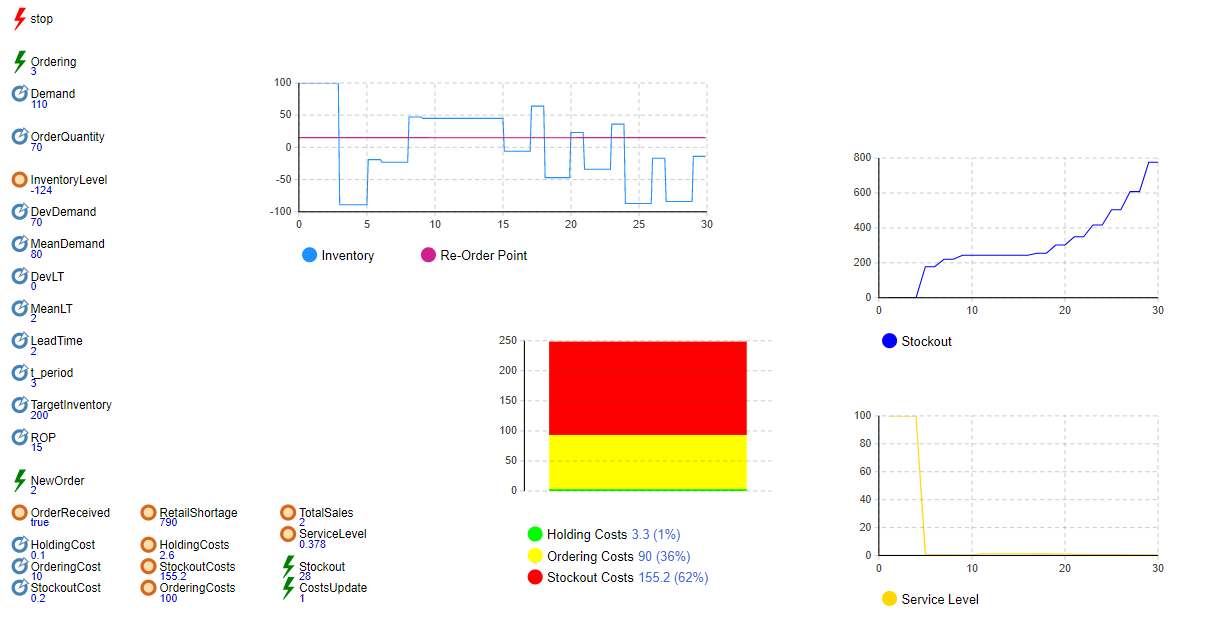
\includegraphics[width=\linewidth]{images/img6invent}
    \caption{Simulación 6. Mismo Escenario con mayor cantidad de demanda.}
\end{figure}

\begin{figure}[H]
    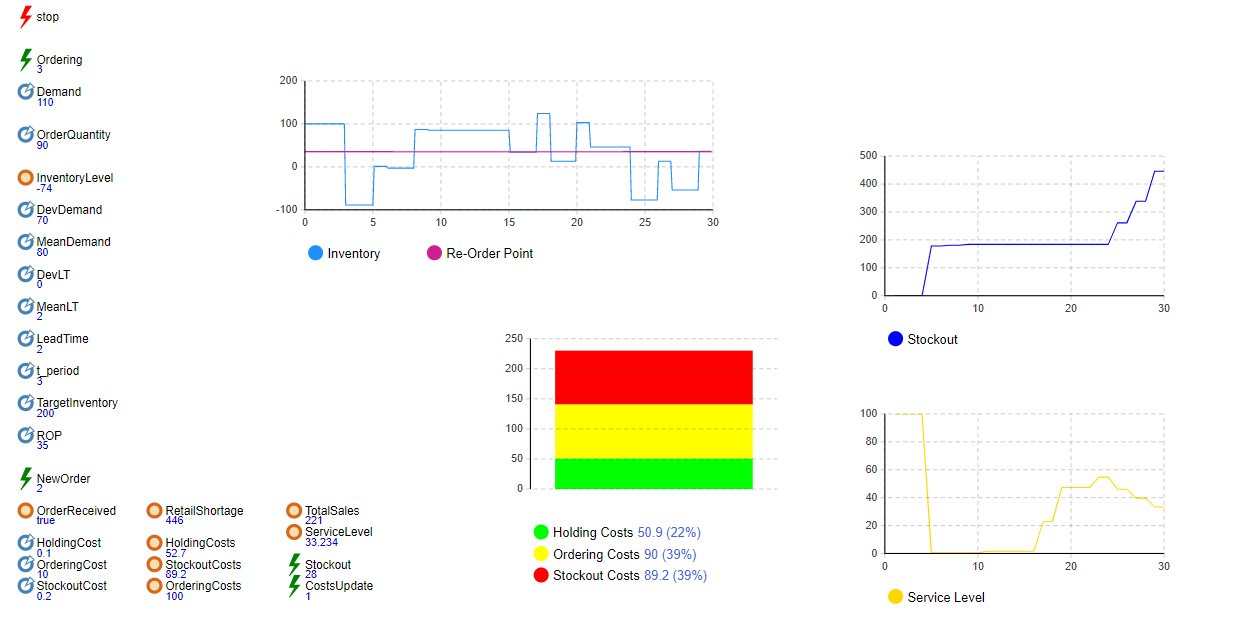
\includegraphics[width=\linewidth]{images/img7invent}
    \caption{Simulación 7. Mismo Escenario con mayor cantidad de orden de compra.}
\end{figure}

\begin{figure}[H]
    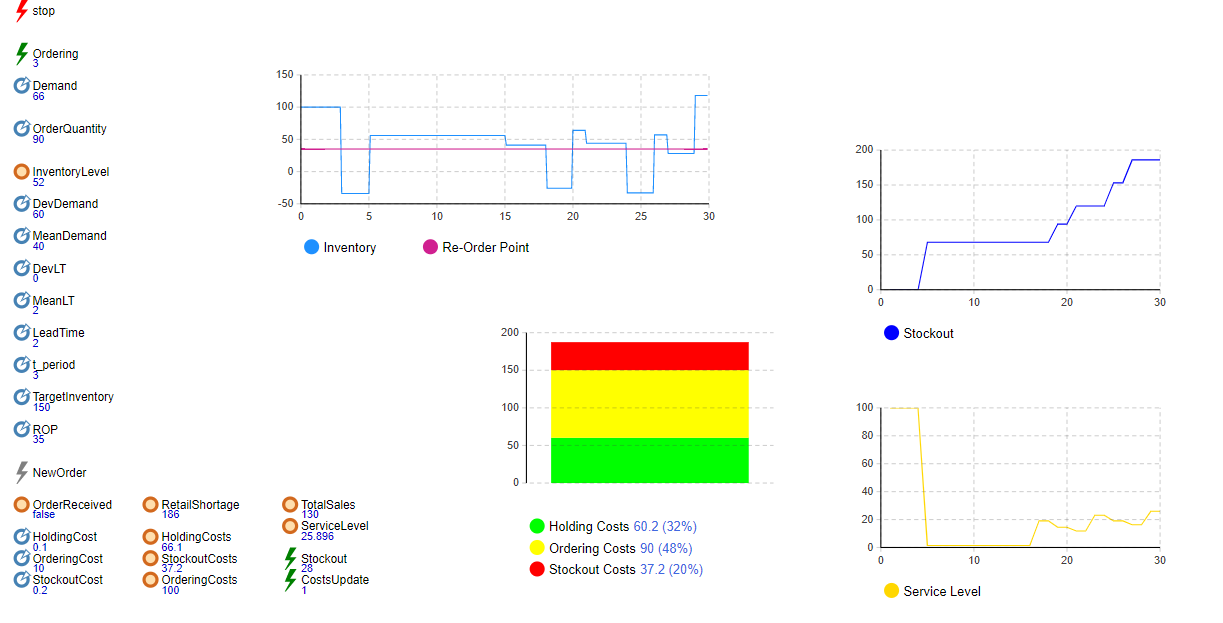
\includegraphics[width=\linewidth]{images/img8invent}
    \caption{Simulación 8. Baja demanda.}
\end{figure}

\begin{figure}[H]
    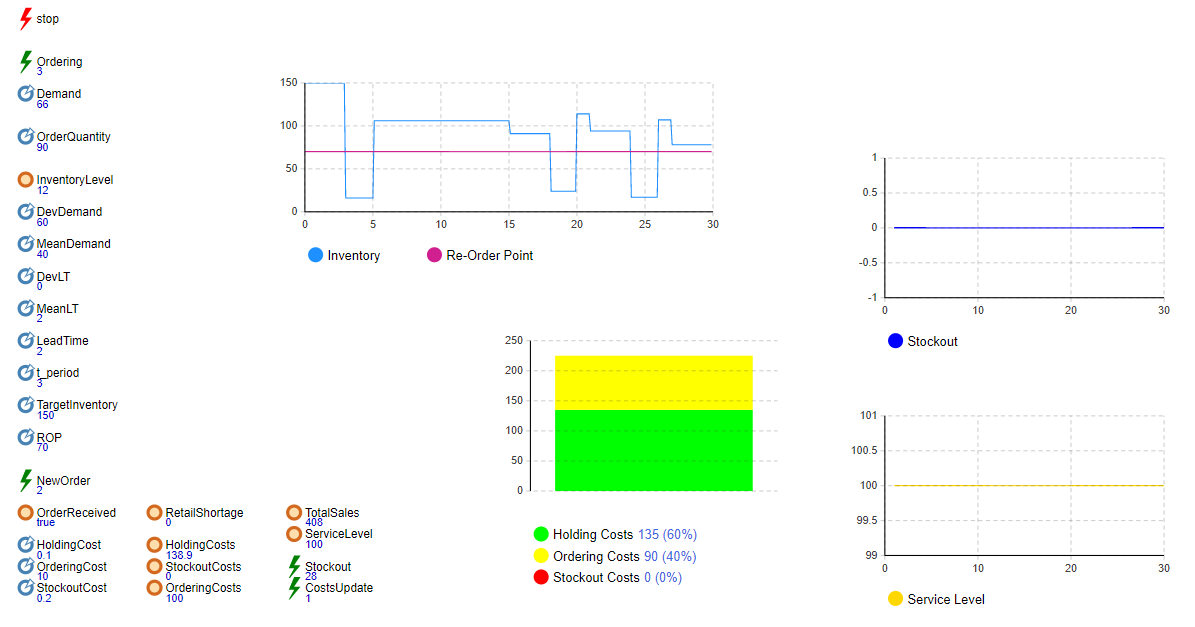
\includegraphics[width=\linewidth]{images/img9invent}
    \caption{Simulación 9. Baja demanda y aumento de ROP.}
\end{figure}

\begin{figure}[H]
    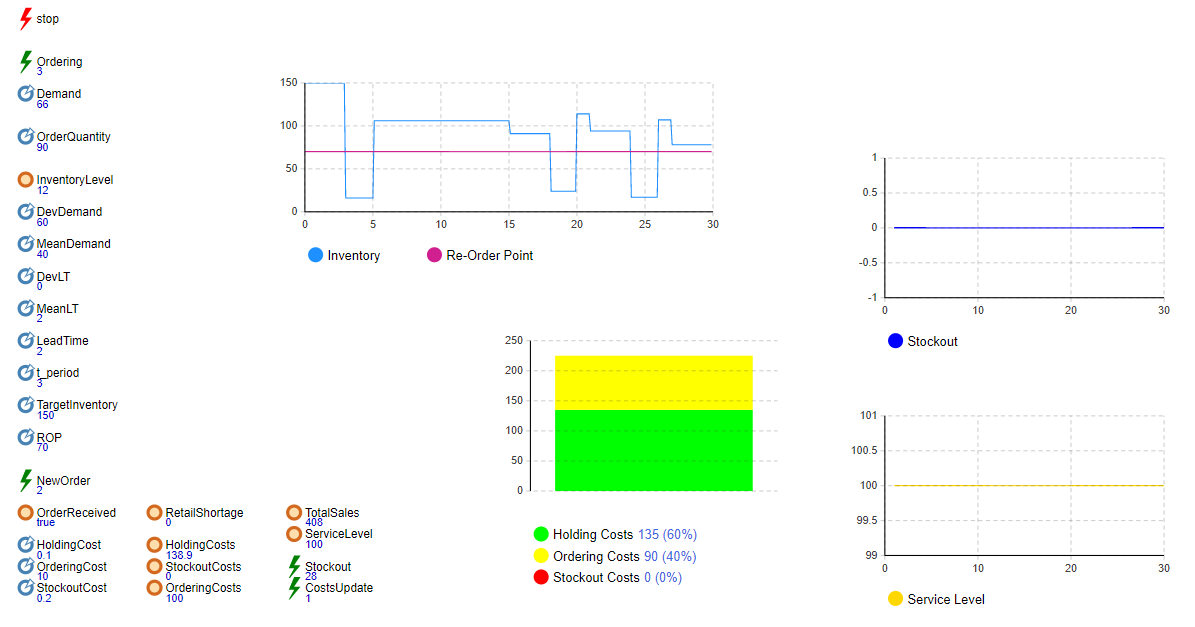
\includegraphics[width=\linewidth]{images/img9invent}
    \caption{Simulación 10. Disminución de orden de compra.}
\end{figure}

\begin{tabular}{||c||c|c|c|c||}
    \hline \hline
    Simulación nro & Orden & Mantenimiento & Faltante & TOTAL\\
    \hline \hline
    1 & $60$ & $486,7$ & $0$ & $546,7$\\
    \hline
    2 & $40$ & $34,8$ & $60,4$ & $135,2$\\
    \hline
    3 & $60$ & $285,5$ & $0$ & $345,5$\\
    \hline
    4 & $40$ & $0$ & $190,8$ & $230,8$\\
    \hline
    5 & $100$ & $0$ & $204,4$ & $304,4$\\
    \hline
    6 & $100$ & $2,6$ & $155,2$ & $257,8$\\
    \hline
    7 & $100$ & $52,7$ & $389,2$ & $541,9$\\
    \hline
    8 & $100$ & $66,1$ & $37,2$ & $203,3$\\
    \hline
    9 & $100$ & $138,9$ & $0$ & $238,9$\\
    \hline
    10 & $100$ & $124,4$ & $0$ &$224,4$\\
    \hline \hline
\end{tabular}

\subsubsection{Conclusion de las simulaciones}\label{subsubsec:conclusiones}
Cabe aclarar que los resultados negativos no significan que se "ahorró" el costo, esto cuenta como 0 debido a que no se pudo realizar el costo de mantenimiento del stock ya que hubo faltante del mismo.
Además se puede observar como en la simulación 2 fué la que más pudo mantener bajos costos a comparación de las demás debido a que tuvo pocas ordenes de compra y una gran existencia al principio.

La Simulación 8 fué la siguiente con menos costo debido a que si bien tuvo muchos gastos en las ordenes de compra, pudo distribuir mejor la faltante y el mantenimiento de la existencia en el inventario.

A su vez la Simulación 1 fué la más costosa, debido a que mantuvo una gran cantidad de stock en el inventario mientras que la segunda mas costosa (la simulación 7) tuvo el mismo problema con la diferencia de que esta que tuvo mucha faltante.

Como conclusión se puede decir que el mayor problema radica en la falta de equilibrio en los costos de cada acción, ya que por ejemplo se pueden tener altos costos de orden de compra, pero esto no fué problema para la simulación 8 que distribuyó la faltante y el mantenimiento de existencia de manera que pudo reducir los costos.
De la misma manera, hubo simulaciones con pocas ordenes de compra pero con altos costes de faltante o de mantenimiento, lo que llevo a grandes costos totales.



\section{Conclusiones}
\label{sec:conclusiones}
Se buscó realizar 10 corridas de cada modelo donde se quizo analizar determinados resultados para saber como se comportaría con parámetros aleatorios.
Ante esto se realizaron los modelos con dos tecnologías distintas para poder compararlas y así tener distintas fuentes de donde evaluar su potencial.
Las tecnologías utilizadas fueron el lenguaje Python, donde se desarrollaron clases y métodos específicos para las corridas;
Y luego se desarrolló el mismo modelo en AnyLogic buscando tener un funcionamiento similar al hecho en código pero a través de patrones específicos de la presente herramienta.

Se puede afirmar que los modelos de simulación creados han funcionado de la manera esperada.
Los creados en Python fueron los más adaptables y maleables debido a la posibilidad de desarrollarlo de la manera más conveniente.
Sin embargo, a pesar de que AnyLogic pueda tener sus restricciones, es una tecnología muy interesante para este tipo de experimentos debido a que cuenta con muchas herramientas que hacen posible llegar a distintas soluciones con una gran capacidad de procesar información y datos.
